\documentclass[11pt,a4paper,]{article}
\usepackage{lmodern}

\usepackage{amssymb,amsmath}
\usepackage{ifxetex,ifluatex}
\usepackage{fixltx2e} % provides \textsubscript
\ifnum 0\ifxetex 1\fi\ifluatex 1\fi=0 % if pdftex
  \usepackage[T1]{fontenc}
  \usepackage[utf8]{inputenc}
\else % if luatex or xelatex
  \usepackage{unicode-math}
  \defaultfontfeatures{Ligatures=TeX,Scale=MatchLowercase}
\fi
% use upquote if available, for straight quotes in verbatim environments
\IfFileExists{upquote.sty}{\usepackage{upquote}}{}
% use microtype if available
\IfFileExists{microtype.sty}{%
\usepackage[]{microtype}
\UseMicrotypeSet[protrusion]{basicmath} % disable protrusion for tt fonts
}{}
\PassOptionsToPackage{hyphens}{url} % url is loaded by hyperref
\usepackage[unicode=true]{hyperref}
\hypersetup{
            pdftitle={Peeking inside FFORMS: Feature-based FORecast Model Selection},
            pdfkeywords={forecasting, time series, machine learning interpretability, black-box
models, LIME},
            pdfborder={0 0 0},
            breaklinks=true}
\urlstyle{same}  % don't use monospace font for urls
\usepackage{geometry}
\geometry{left=2.5cm,right=2.5cm,top=2.5cm,bottom=2.5cm}
\usepackage[style=authoryear-comp,]{biblatex}
\addbibresource{references.bib}
\usepackage{longtable,booktabs}
% Fix footnotes in tables (requires footnote package)
\IfFileExists{footnote.sty}{\usepackage{footnote}\makesavenoteenv{long table}}{}
\usepackage{graphicx,grffile}
\makeatletter
\def\maxwidth{\ifdim\Gin@nat@width>\linewidth\linewidth\else\Gin@nat@width\fi}
\def\maxheight{\ifdim\Gin@nat@height>\textheight\textheight\else\Gin@nat@height\fi}
\makeatother
% Scale images if necessary, so that they will not overflow the page
% margins by default, and it is still possible to overwrite the defaults
% using explicit options in \includegraphics[width, height, ...]{}
\setkeys{Gin}{width=\maxwidth,height=\maxheight,keepaspectratio}
\IfFileExists{parskip.sty}{%
\usepackage{parskip}
}{% else
\setlength{\parindent}{0pt}
\setlength{\parskip}{6pt plus 2pt minus 1pt}
}
\setlength{\emergencystretch}{3em}  % prevent overfull lines
\providecommand{\tightlist}{%
  \setlength{\itemsep}{0pt}\setlength{\parskip}{0pt}}
\setcounter{secnumdepth}{5}

% set default figure placement to htbp
\makeatletter
\def\fps@figure{htbp}
\makeatother


\title{Peeking inside FFORMS: Feature-based FORecast Model Selection}

%% MONASH STUFF

%% CAPTIONS
\RequirePackage{caption}
\DeclareCaptionStyle{italic}[justification=centering]
 {labelfont={bf},textfont={it},labelsep=colon}
\captionsetup[figure]{style=italic,format=hang,singlelinecheck=true}
\captionsetup[table]{style=italic,format=hang,singlelinecheck=true}

%% FONT
\RequirePackage{bera}
\RequirePackage{mathpazo}

%% HEADERS AND FOOTERS
\RequirePackage{fancyhdr}
\pagestyle{fancy}
\rfoot{\Large\sffamily\raisebox{-0.1cm}{\textbf{\thepage}}}
\makeatletter
\lhead{\textsf{\expandafter{\@title}}}
\makeatother
\rhead{}
\cfoot{}
\setlength{\headheight}{15pt}
\renewcommand{\headrulewidth}{0.4pt}
\renewcommand{\footrulewidth}{0.4pt}
\fancypagestyle{plain}{%
\fancyhf{} % clear all header and footer fields
\fancyfoot[C]{\sffamily\thepage} % except the center
\renewcommand{\headrulewidth}{0pt}
\renewcommand{\footrulewidth}{0pt}}

%% MATHS
\RequirePackage{bm,amsmath}
\allowdisplaybreaks

%% GRAPHICS
\RequirePackage{graphicx}
\setcounter{topnumber}{2}
\setcounter{bottomnumber}{2}
\setcounter{totalnumber}{4}
\renewcommand{\topfraction}{0.85}
\renewcommand{\bottomfraction}{0.85}
\renewcommand{\textfraction}{0.15}
\renewcommand{\floatpagefraction}{0.8}

%\RequirePackage[section]{placeins}

%% SECTION TITLES
\RequirePackage[compact,sf,bf]{titlesec}
\titleformat{\section}[block]
  {\fontsize{15}{17}\bfseries\sffamily}
  {\thesection}
  {0.4em}{}
\titleformat{\subsection}[block]
  {\fontsize{12}{14}\bfseries\sffamily}
  {\thesubsection}
  {0.4em}{}
\titlespacing{\section}{0pt}{*5}{*1}
\titlespacing{\subsection}{0pt}{*2}{*0.2}


%% TITLE PAGE
\def\Date{\number\day}
\def\Month{\ifcase\month\or
 January\or February\or March\or April\or May\or June\or
 July\or August\or September\or October\or November\or December\fi}
\def\Year{\number\year}

\makeatletter
\def\wp#1{\gdef\@wp{#1}}\def\@wp{??/??}
\def\jel#1{\gdef\@jel{#1}}\def\@jel{??}
\def\showjel{{\large\textsf{\textbf{JEL classification:}}~\@jel}}
\def\nojel{\def\showjel{}}
\def\addresses#1{\gdef\@addresses{#1}}\def\@addresses{??}
\def\cover{{\sffamily\setcounter{page}{0}
        \thispagestyle{empty}
        \placefig{2}{1.5}{width=5cm}{monash2}
        \placefig{16.9}{1.5}{width=2.1cm}{MBusSchool}
        \begin{textblock}{4}(16.9,4)ISSN 1440-771X\end{textblock}
        \begin{textblock}{7}(12.7,27.9)\hfill
        
\includegraphics[height=0.7cm]{AACSB}~~~
        
\includegraphics[height=0.7cm]{EQUIS}~~~
        
\includegraphics[height=0.7cm]{AMBA}
        \end{textblock}
        \vspace*{2cm}
        \begin{center}\Large
        Department of Econometrics and Business Statistics\\[.5cm]
        \footnotesize http://monash.edu/business/ebs/research/publications
        \end{center}\vspace{2cm}
        \begin{center}
        \fbox{\parbox{14cm}{\begin{onehalfspace}\centering\Huge\vspace*{0.3cm}
                \textsf{\textbf{\expandafter{\@title}}}\vspace{1cm}\par
                \LARGE\@author\end{onehalfspace}
        }}
        \end{center}
        \vfill
                \begin{center}\Large
                \Month~\Year\\[1cm]
                Working Paper \@wp
        \end{center}\vspace*{2cm}}}
\def\pageone{{\sffamily\setstretch{1}%
        \thispagestyle{empty}%
        \vbox to \textheight{%
        \raggedright\baselineskip=1.2cm
     {\fontsize{24.88}{30}\sffamily\textbf{\expandafter{\@title}}}
        \vspace{2cm}\par
        \hspace{1cm}\parbox{14cm}{\sffamily\large\@addresses}\vspace{1cm}\vfill
        \hspace{1cm}{\large\Date~\Month~\Year}\\[1cm]
        \hspace{1cm}\showjel\vss}}}
\def\blindtitle{{\sffamily
     \thispagestyle{plain}\raggedright\baselineskip=1.2cm
     {\fontsize{24.88}{30}\sffamily\textbf{\expandafter{\@title}}}\vspace{1cm}\par
        }}
\def\titlepage{{\cover\newpage\pageone\newpage\blindtitle}}

\def\blind{\def\titlepage{{\blindtitle}}\let\maketitle\blindtitle}
\def\titlepageonly{\def\titlepage{{\pageone\end{document}}}}
\def\nocover{\def\titlepage{{\pageone\newpage\blindtitle}}\let\maketitle\titlepage}
\let\maketitle\titlepage
\makeatother

%% SPACING
\RequirePackage{setspace}
\spacing{1.5}

%% LINE AND PAGE BREAKING
\sloppy
\clubpenalty = 10000
\widowpenalty = 10000
\brokenpenalty = 10000
\RequirePackage{microtype}

%% PARAGRAPH BREAKS
\setlength{\parskip}{1.4ex}
\setlength{\parindent}{0em}

%% HYPERLINKS
\RequirePackage{xcolor} % Needed for links
\definecolor{darkblue}{rgb}{0,0,.6}
\RequirePackage{url}

\makeatletter
\@ifpackageloaded{hyperref}{}{\RequirePackage{hyperref}}
\makeatother
\hypersetup{
     citecolor=0 0 0,
     breaklinks=true,
     bookmarksopen=true,
     bookmarksnumbered=true,
     linkcolor=darkblue,
     urlcolor=blue,
     citecolor=darkblue,
     colorlinks=true}

%% KEYWORDS
\newenvironment{keywords}{\par\vspace{0.5cm}\noindent{\sffamily\textbf{Keywords:}}}{\vspace{0.25cm}\par\hrule\vspace{0.5cm}\par}

%% ABSTRACT
\renewenvironment{abstract}{\begin{minipage}{\textwidth}\parskip=1.4ex\noindent
\hrule\vspace{0.1cm}\par{\sffamily\textbf{\abstractname}}\newline}
  {\end{minipage}}


\usepackage[T1]{fontenc}
\usepackage[utf8]{inputenc}

\usepackage[showonlyrefs]{mathtools}
\usepackage[no-weekday]{eukdate}

%% BIBLIOGRAPHY

\makeatletter
\@ifpackageloaded{biblatex}{}{\usepackage[style=authoryear-comp, backend=biber, natbib=true]{biblatex}}
\makeatother
\ExecuteBibliographyOptions{bibencoding=utf8,minnames=1,maxnames=3, maxbibnames=99,dashed=false,terseinits=true,giveninits=true,uniquename=false,uniquelist=false,doi=false, isbn=false,url=true,sortcites=false}

\DeclareFieldFormat{url}{\texttt{\url{#1}}}
\DeclareFieldFormat[article]{pages}{#1}
\DeclareFieldFormat[inproceedings]{pages}{\lowercase{pp.}#1}
\DeclareFieldFormat[incollection]{pages}{\lowercase{pp.}#1}
\DeclareFieldFormat[article]{volume}{\mkbibbold{#1}}
\DeclareFieldFormat[article]{number}{\mkbibparens{#1}}
\DeclareFieldFormat[article]{title}{\MakeCapital{#1}}
\DeclareFieldFormat[inproceedings]{title}{#1}
\DeclareFieldFormat{shorthandwidth}{#1}
% No dot before number of articles
\usepackage{xpatch}
\xpatchbibmacro{volume+number+eid}{\setunit*{\adddot}}{}{}{}
% Remove In: for an article.
\renewbibmacro{in:}{%
  \ifentrytype{article}{}{%
  \printtext{\bibstring{in}\intitlepunct}}}

\makeatletter
\DeclareDelimFormat[cbx@textcite]{nameyeardelim}{\addspace}
\makeatother
\renewcommand*{\finalnamedelim}{%
  %\ifnumgreater{\value{liststop}}{2}{\finalandcomma}{}% there really should be no funny Oxford comma business here
  \addspace\&\space}


\wp{no/yr}
\jel{C10,C14,C22}

\RequirePackage[absolute,overlay]{textpos}
\setlength{\TPHorizModule}{1cm}
\setlength{\TPVertModule}{1cm}
\def\placefig#1#2#3#4{\begin{textblock}{.1}(#1,#2)\rlap{\includegraphics[#3]{#4}}\end{textblock}}



\blind



\date{\sf\Date~\Month~\Year}
\makeatletter
 \lfoot{\sf\@date}
\makeatother

%% Any special functions or other packages can be loaded here.
%% Any special functions or other packages can be loaded here.
\usepackage{tikz}
\usepackage{algorithm}
\usepackage{algpseudocode}
\usepackage{amsthm}
\usepackage{amsmath,bm}
\usepackage{paralist}
\usepackage{todonotes}
\usepackage{ctable}
\usepackage{multirow}
\usepackage{lscape}
\usepackage{rotating}
\usepackage{float} 
\floatplacement{figure}{H} 

\def\sectionautorefname{Section}
\captionsetup[figure]{font=small}
\captionsetup[table]{font=small}
\def\var{\text{Var}}
\allowdisplaybreaks
\sloppy

%% LINE AND PAGE BREAKING
\clubpenalty = 4500
\widowpenalty = 4500
\brokenpenalty = 4500


\def\yes{$\checkmark$}

\setlength{\abovedisplayskip}{5pt}
\setlength{\belowdisplayskip}{5pt}
\setlength{\abovedisplayshortskip}{0pt}
\setlength{\belowdisplayshortskip}{0pt}


\begin{document}
\maketitle
\begin{abstract}
Features of time series are useful in identifying suitable models for
forecasting. Talagala, Hyndman \& Athanasopoulos (2018) proposed a
classification framework, labelled FFORMS (Feature-based FORecast Model
Selection), which selects forecast models based on features calculated
from the time series. The FFORMS framework builds a mapping that relates
the features of a time series to the ``best'' forecast model using a
random forest. In this paper we explore what is happening under the hood
of the FFORMS framework. This is accomplished using model-agnostic
machine learning interpretability approaches. The analysis provides a
valuable insight into how different features and their interactions
affect the choice of forecast model.
\end{abstract}
\begin{keywords}
forecasting, time series, machine learning interpretability, black-box
models, LIME
\end{keywords}

\section{Introduction}\label{intro}

The field of time series forecasting has been evolving for a few decades
now and has introduced a wide variety of models for forecasting.
However, for a given time series the selection of an appropriate
forecast-model among many possibilities is not straight forward. This
selection is one of the most difficult tasks as each method perform best
for some but not all tasks. The features of a time series are considered
to be an important factor in identifying suitable forecasting models
\autocites{collopy1992rule}{meade2000evidence}{makridakis2000m3}{wang2009rule}.
However, a comprehensive description of the relationship between the
features and the performance of algorithms is rarely discussed.

There have been several recent studies on the use of meta-learning
approaches to automate forecast-model selection based on features
computed from the time series
\autocites{shah1997model}{prudencio2004meta}{lemke2010meta}{kuck2016meta}.
A meta-learning approach provides a systematic guidance on model
selection based on knowledge acquired from historical data sets. The key
idea is, forecast-model selection is posed as a supervised learning
task. Each time series in the meta-data set is represented as a vector
of features and labelled according to the ``best'' forecast-model
(i.e.~for example model with lowest MASE over a test set, etc.). Then a
meta-learner is trained to identify a suitable forecast-model (usually a
machine learning algorithm is used). In the era of big data, such an
automated model selection process is necessary because the cost of
invoking all possible forecast-models is prohibitive. However, the
existing literature suffers from the limitation of providing answers to
questions such as: i) How features are related to the property being
modelled?; ii) How features interact with each other to identify a
suitable forecast-model?; iii) Which features contribute most to the
classification process? etc. Addressing such questions can enhance the
understanding of the relations between features and model selection
outcomes. To the best of our knowledge, a very limited effort has been
taken to understand how the meta-learners are making its decisions and
what is really happening inside these complex model structures.
Providing transparency will result, building trust in the prediction
results of the meta-learner.

Furthermore, besides the goal of developing an automated forecast-model
selection framework very few researchers have made an attempt to provide
a description of the relationship between the features and the choice of
different forecast-models
\autocites{schnaars1984situational}{wang2009rule}{lemke2010meta}[ are
among some exceptions]{petropoulos2014horses}. These studies are limited
by the scale of problem instances used, the diversity of forecast-models
implemented, and the limited number of features considered to identify
the relationship between features and forecast-model performance.

To fill this gap, this paper makes a first step towards providing a
comprehensive analysis of the relationship between time series features
and forecast-model selection using machine learning interpretability
techniques. This paper builds on the method from our previous work
\textcite{fforms}, in which we introduced the FFORMS (Feature-based
FORecast Model Selection) framework. A random forest is used to model
the relationship between features and ``best'' performing
forecast-model. A large collection of time series is used to train the
meta-learner.

In this article, we make the following contributions:

\begin{enumerate}
\def\labelenumi{\arabic{enumi}.}
\tightlist
\item
  We extend the FFORMS framework to handle weekly, daily and hourly
  series. We also extend the diversity of forecast-models used as class
  labels. The contribution of this paper differs from previously
  published work related to meta-learning
  \autocites{prudencio2004meta}{lemke2010meta}{kuck2016meta} in three
  ways: i) a more extensive collection of features is used (35 different
  feature types are used which are simple and easy to compute), ii) the
  diversity of forecast-models considered as class labels, and iii)
  capability of handling high frequency data;
\item
  We analyse the application of the FFORMS framework to the
  M4-competition data. We generated point forecasts and prediction
  intervals for the M4-competition time series data, and is shown to
  yield accurate forecast comparable to several benchmarks and other
  commonly used automated approaches of time series forecasting. Our
  approach achieved a high accuracy rate based on individual
  forecast-model selection rule.
\item
  The main contribution of the paper is to explore the relationship
  between features of time series and the choice of forecast-model
  selection using the FFORMS framework. We explore the role of features
  in two different perspectives: i) Global perspective of feature
  contribution: the overall role of features in the choice of different
  forecast-models and ii) Local perspective of feature contribution: we
  zoom into local regions of the data to identify which features
  contribute most to classify a specific instance. In this category we
  make five fundamental contributions. They are,

  \begin{enumerate}
  \def\labelenumii{\roman{enumii})}
  \tightlist
  \item
    visualise patterns leaned by the meta-leaner
  \item
    rank features according to their importance in the choice of
    forecast-model selection and identify which features are
    contributing mostly to the predictive mechanism of the fitted model.
  \item
    visualise learned relationships between features and the choice of
    forecast-model selection using partial dependence plots introduced
    by \textcite{friedman2008predictive}.
  \item
    Assessment of interaction effect between features
  \item
    visualise regions in the feature-space in which good or exceptional
    performance is expected from different forecast-models.
  \end{enumerate}
\end{enumerate}

The remainder of the paper is structured as follows. The
\autoref{fforms} outlines the extended FFORMS framework.
\autoref{offline} through \autoref{peeking} explain the three main
components of the extended FFORMS framework. In \autoref{results} we
discuss the results. \autoref{conclusions} concludes.

\section{Methodological framework}\label{fforms}

\autoref{fig:framework} shows the extended FFORMS framework with all
additional components highlighted in yellow. There are three main
components of this extended FFORMS framework. They are,

\begin{enumerate}
\def\labelenumi{\arabic{enumi}.}
\tightlist
\item
  offline phase (blue):, the development of a meta-learner
\item
  online phase (red): use the pre-trained meta-learner to identify the
  ``best'' forecast-model.
\item
  peeking inside FFORMS (yellow): gain insights into what what is
  happening under the hood of the FFORMS framework.
\end{enumerate}

We now explain application of the extended FFORMS framework to the
M4-competition data. We analyse yearly, quarterly, monthly, weekly,
daily and hourly series separately due to their differences in
frequencies and hence the appropriateness of different features and
forecast-models we considered as class labels.

\begin{figure}[h]
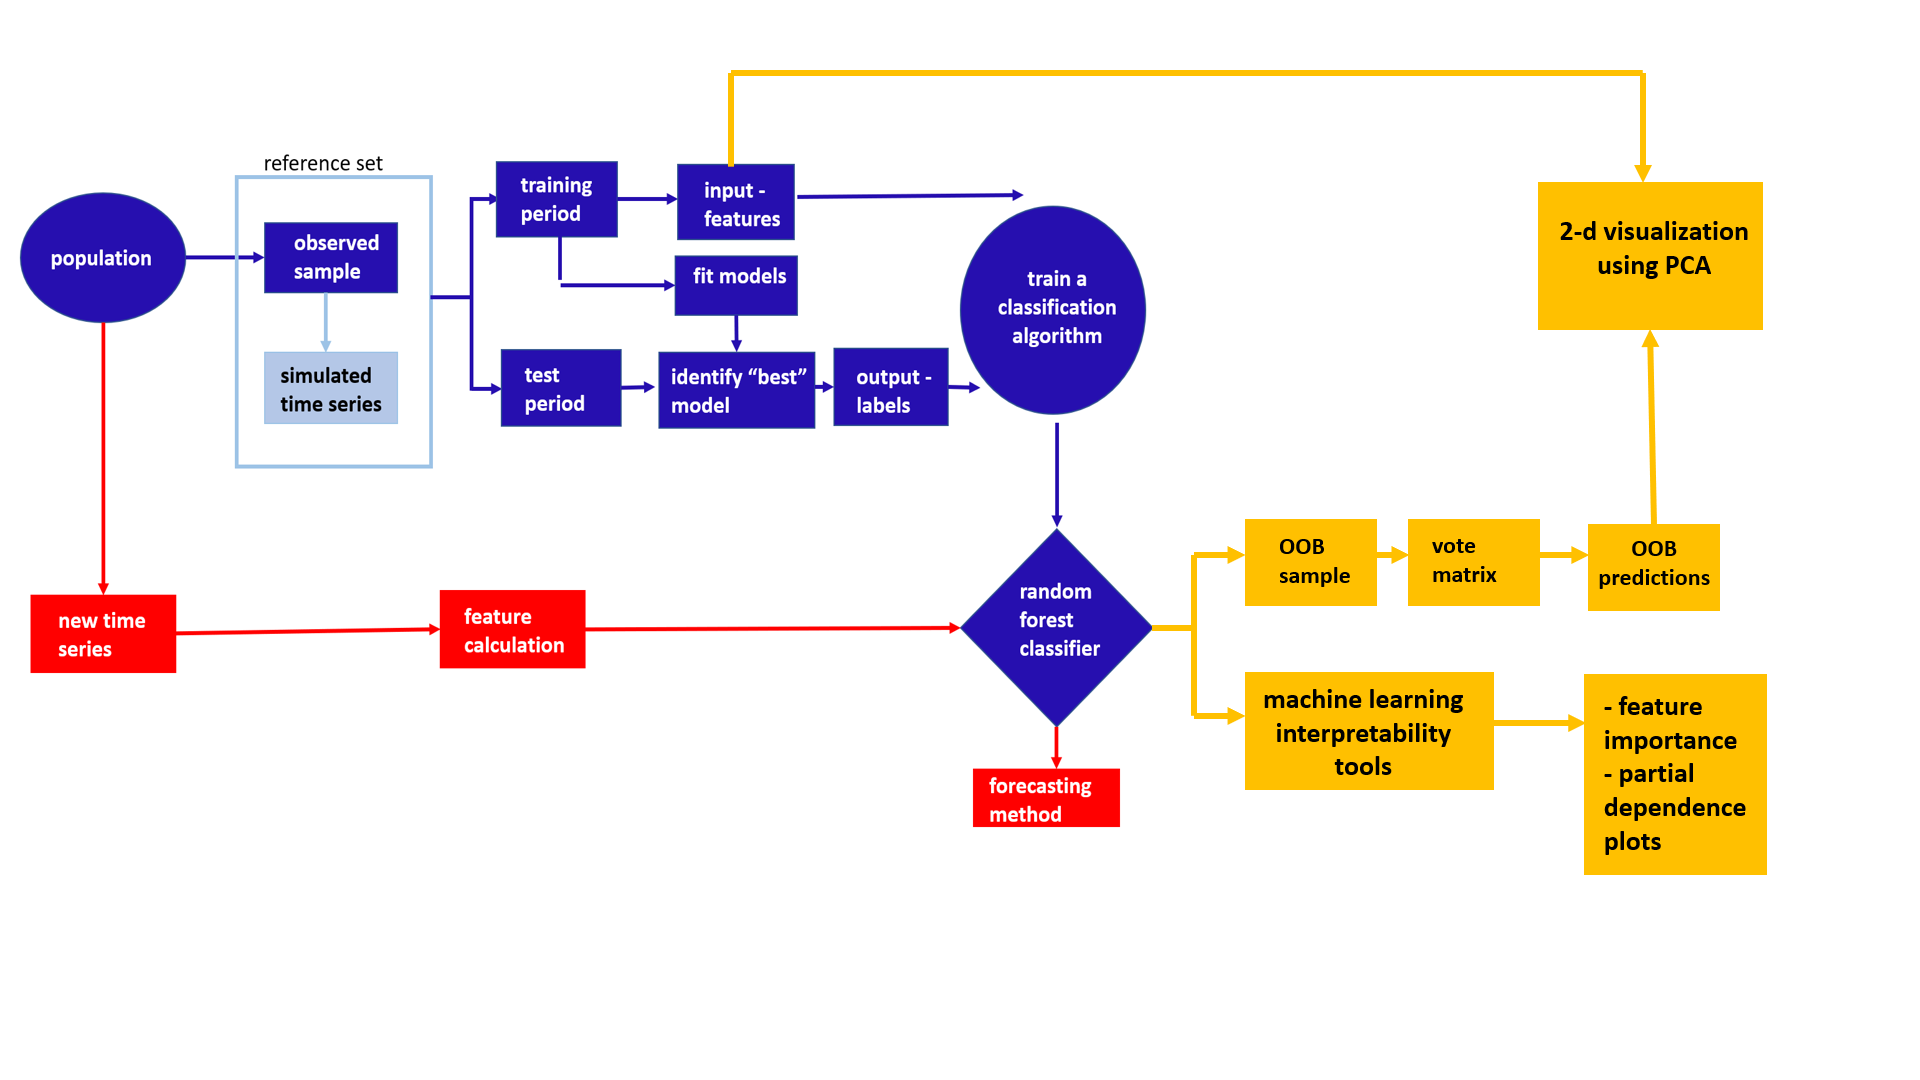
\includegraphics[width=1.15\linewidth]{figures/framework} \caption{extended FFORMS (Feature-based FORecast-Model Selection) framework. The offline phase is shown in blue, the online phase by red and the peeking inside FFORMS is shown in yellow.}\label{fig:framework}
\end{figure}

\section{Offline phase}\label{offline}

\subsection{Reference set}\label{reference-set}

We call the collection of time series used for training the meta-leaner
as the ``reference set''. The reference set consist of two sets of time
series: i) observed sample and ii) simulated time series.

\subsubsection{Observed sample}\label{observed-sample}

We use the time series from the M1, M3 and M4 competitions as the
observed sample. Table \ref{observedsample} summarizes the number of
time series in the observed sample. Note that from the M4 competition a
randomly selected subset of time series are used for the observed
sample. The rest shown by the column labelled ``Test set - M4'' are used
as a validation set to evaluate the performance of the meta-learner.

\begin{table}[!h]
\centering
\caption{Composition of the time series in the observed sample and the test set}
\label{observedsample}
\begin{tabular}{l|rrr|r}
\multirow{2}{*}{Frequency} & \multicolumn{3}{l|}{Observed Sample} & Test set \\
&   M1    &    M3   &    M4 & M4 \\ \hline
Yearly          &   181    &   645    &   22000 & 1000 \\
Quarterly       &   203    &    756   &   23000 & 1000\\
Monthly         &   617    &    1428   &  47000 & 1000\\
Weekly          &   -    &   -    &   259 & 100\\
Daily           &   -    &   -    &   4001 & 226\\
Hourly          &   -    &    -   &  350 & 64\\ \hline
\end{tabular}
\end{table}

\subsubsection{Simulated time series}\label{simulated-time-series}

As described in \textcite{fforms}, we augment the reference set by
adding multiple time series simulated based on each series in the M4
competition. We use several automated algorithms to simulate multiple
time series. Table \ref{simulation} shows the data generating algorithms
used for each frequency. The \texttt{ets()} and \texttt{auto.arima()}
functions available in the forecast package in R \autocite{forecast} are
used to simulate yearly, quarterly and monthly data from exponential
smoothing and ARIMA models. The \texttt{stlf()} function also available
in the forecast package is used to simulate multiple time series based
on multiple seasonal decomposition approach. Using the above functions,
we fit models to each time series in the M4 database and then simulate
multiple time series from the selected models. In this experiment the
length of the simulated time series is set to be equal to: length of the
training period specified in the M4 competition + length of the forecast
horizon specified in the competition. For example, the series with id
``Y13190'' contains a training period of length 835. The length of the
simulated series generated based on this series is equals to 841
(835+6). Before simulating time series from daily and hourly series, we
convert the time series into multiple seasonal time series (msts)
objects. For daily time series with length less than 366, the frequency
set to 7 and longer time series are converted to multiple seasonal time
series objects with frequencies set to 7 and 365.25. For hourly series,
we set the frequencies to 24 and 168 to handle multiple frequencies
corresponds to time-of-day pattern and time-of-week pattern
respectively.

\begin{table}[!h]
\centering
\caption{Automatic forecasting algorithms used to simulate time series}
\label{simulation}
\begin{tabular}{lllllll}
Algorithm & Y & Q & M & W & D &  H \\ \hline
ets() & \checkmark & \checkmark & \checkmark &  &  &  \\
auto.arima() & \checkmark & \checkmark & \checkmark &  &  &  \\
stlf() &  &  &  & \checkmark & \checkmark & \checkmark\\ \hline
\end{tabular}
\end{table}

We should re-emphasize that all the observed time series and the
simulated time series form the reference set to build our meta-learner.
Once we create the reference set for random forest training we split
each time series in the reference set into training period and test
period.

\subsection{Input: features}\label{input-features}

The FFORMS framework operates on features calculated from the time
series. For each time series in the reference set, features are
calculated based on the training period of the time series.

\begin{table}[!htp]
\centering\footnotesize\tabcolsep=0.12cm
\caption{Time series features}
\label{feature}
\begin{tabular}{llp{8,8cm}cccc}
\toprule
\multicolumn{2}{c}{Feature} & Description & Y & Q/M & W & D/H\\
\midrule
1  & T              & length of time series                                                                   & \yes  & \yes & \yes & \yes\\
2  & trend          & strength of trend                                                                       & \yes  & \yes & \yes & \yes\\
3  & seasonality 1    & strength of seasonality corresponds to frequency 1                                                              & -     & \yes & \yes & \yes\\
4  & seasonality 2    & strength of seasonality corresponds to frequency 2                                                              & -     & - & -& \yes\\
5  & linearity      & linearity                                                                               & \yes  & \yes & \yes & \yes\\
6  & curvature      & curvature                                                                               & \yes  & \yes & \yes & \yes\\
7  & spikiness      & spikiness                                                                               & \yes  & \yes & \yes & \yes\\
8  & e\_acf1        & first ACF value of remainder series                                                     & \yes  & \yes & \yes & \yes\\
9  & stability      & stability                                                                               & \yes  & \yes & \yes & \yes\\
10  & lumpiness      & lumpiness                                                                               & \yes  & \yes & \yes & \yes\\
11 & entropy        & spectral entropy                                                                        & \yes  & \yes & \yes & \yes\\
12 & hurst          & Hurst exponent                                                                          & \yes  & \yes & \yes & \yes\\
13 & nonlinearity   & nonlinearity                                                                            & \yes\ & \yes & \yes & \yes\\
14 & alpha          & ETS(A,A,N) $\hat\alpha$                                                                 & \yes  & \yes & \yes & -\\
15 & beta           & ETS(A,A,N) $\hat\beta$                                                                  & \yes  & \yes & \yes & - \\
16 & hwalpha        & ETS(A,A,A) $\hat\alpha$                                                                 & -     & \yes & - & -\\
17 & hwbeta         & ETS(A,A,A) $\hat\beta$                                                                  & -     & \yes & - & - \\
18 & hwgamma        & ETS(A,A,A) $\hat\gamma$                                                                 & -     & \yes & - &-\\
19 & ur\_pp         & test statistic based on Phillips-Perron test                                            & \yes  & - & - & - \\
20 & ur\_kpss       & test statistic based on KPSS test                                                       & \yes  & - & - & - \\
21 & y\_acf1        & first ACF value of the original series                                                  & \yes  & \yes & \yes & \yes\\
22 & diff1y\_acf1   & first ACF value of the differenced series                                               & \yes  & \yes & \yes & \yes\\
23 & diff2y\_acf1   & first ACF value of the twice-differenced series                                         & \yes  & \yes & \yes & \yes\\
24 & y\_acf5        & sum of squares of first 5 ACF values of original series                                 & \yes  & \yes & \yes & \yes\\
25 & diff1y\_acf5   & sum of squares of first 5 ACF values of differenced series                              & \yes  & \yes & \yes & \yes\\
26 & diff2y\_acf5   & sum of squares of first 5 ACF values of twice-differenced series                        & \yes  & \yes & \yes & \yes \\
27 & seas\_acf1     & autocorrelation coefficient at first seasonal lag                                       & -     & \yes & \yes & \yes\\
28 & sediff\_acf1   & first ACF value of seasonally-differenced series                                        & -     & \yes & \yes & \yes\\
29 & sediff\_seacf1 & ACF value at the first seasonal lag of seasonally-differenced series                    & -     & \yes & \yes & \yes\\
30 & sediff\_acf5   & sum of squares of first 5 autocorrelation coefficients of seasonally-differenced series & -     & \yes & \yes & \yes\\
31 & seas\_pacf     & partial autocorrelation coefficient at first seasonal lag & -     & \yes & \yes & \yes\\
32 & lmres\_acf1    & first ACF value of residual series of linear trend model                                & \yes  & - & - & -\\
33 & y\_pacf5       & sum of squares of first 5 PACF values of original series                                & \yes  & \yes & \yes & \yes\\
34 & diff1y\_pacf5  & sum of squares of first 5 PACF values of differenced series                             & \yes  & \yes & \yes & \yes\\
35 & diff2y\_pacf5  & sum of squares of first 5 PACF values of twice-differenced series                       & \yes  & \yes & \yes & \yes\\
\bottomrule
\end{tabular}
\end{table}

The description of the features calculated under each frequency category
is shown in Table \ref{feature}. A comprehensive description of the
features used in the experiment is given in \textcite{fforms}.

\subsection{Output: class-labels}\label{output-class-labels}

The description of class labels considered under each frequency is shown
in Table \ref{classlabels}. Note that these added to \textcite{fforms}.
Most of the labels given in Table \ref{classlabels} are self-explanatory
labels. In STL-AR, mstlets, and mstlarima, first an STL decomposition is
applied to the time series and then seasonal naive is used to forecast
the seasonal component. Then, AR, ETS and ARIMA models are used to
forecast the seasonally adjusted data respectively. We fit the
corresponding models outlined in Table \ref{classlabels} to each series
in the reference set. The models are estimated using the training period
for each series, and forecasts are produced for the test periods.

\begin{table}[!htp]
\centering\footnotesize\tabcolsep=0.12cm
\caption{Class labels}
\label{classlabels}
\begin{tabular}{llrrrr}
class label & Description & Y & Q/M & W & D/H \\ \hline
WN & white noise process & \checkmark & \checkmark & \checkmark & \checkmark \\
AR/MA/ARMA & AR, MA, ARMA processes & \checkmark & \checkmark & \checkmark & -\\
ARIMA & ARIMA process & \checkmark & \checkmark & \checkmark & - \\
SARIMA & seasonal ARIMA & \checkmark & \checkmark & \checkmark & -\\
RWD & random walk with drift & \checkmark & \checkmark & \checkmark & \checkmark \\
RW & random walk & \checkmark & \checkmark & \checkmark & \checkmark  \\
Theta & standard theta method & \checkmark & \checkmark & \checkmark & \checkmark \\
STL-AR &  & - & \checkmark & \checkmark & \checkmark \\
ETS-notrendnoseasonal & ETS without trend and seasonal components & \checkmark & \checkmark & \checkmark & - \\
ETStrendonly & ETS with trend component and without seasonal component & \checkmark & \checkmark & \checkmark & -\\
ETSdampedtrend & ETS with damped trend component and without seasonal component  & \checkmark &  \checkmark & - & - \\
ETStrendseasonal & ETS with trend and seasonal components & - & \checkmark & - & - \\
ETSdampedtrendseasonal & ETS with damped trend and seasonal components & - & \checkmark & - & -\\
ETSseasonalonly & ETS with seasonal components and without trend component & -  & \checkmark & - & - \\
snaive & seasonal naive method & \checkmark & \checkmark & \checkmark & \checkmark \\
tbats & TBATS forecasting & - & \checkmark & \checkmark & \checkmark \\
nn & neural network time series forecasts & \checkmark & \checkmark & \checkmark & \checkmark \\
mstlets &  & - & - & \checkmark & \checkmark \\
mstlarima & & - & - & - & \checkmark \\\hline
\end{tabular}
\end{table}

According to the \textcite{M4compguide}, in the M4-competition the
forecast accuracy is evaluated based on the mean Absolute Scaled Error
(MASE) and the symmetric Mean Absolute Percentage Error (MAPE). Hence,
in order to identify the ``best'' forecast-model for each time series in
the reference set we combine MASE and the symmetric MAPE calculated over
the test set. More specifically, for each series both forecast error
measures MASE and sMAPE are calculated for each of the forecast models.
Each of these is respectively standardized by the median MASE and median
sMAPE calculated across the forecast-models. The model with the lowest
average value of the scaled MASE and scaled sMAPE is selected as the
output class-label.

The last step of offline phase of the framewok is to train a
meta-learner. A random forest algorithm is used to train the
meta-learner.

\section{Online phase}\label{online}

The online phase of the algorithm involves generating point forecasts
and 95\% prediction intervals for the new series or the future values
observed time series. First, the corresponding features are calculated
based on the full length of the training period provided by the M4
competition. Second, point forecasts and 95\% prediction intervals are
calculated based on the predicted class labels. We should note that all
negative forecasts are set to zero.

\section{Peeking inside FFORMS}\label{peeking}

The main objective of this paper is to explore the nature of the
relationship between features and forecast-model selection learned by
the FFORMS framework. More specifically, to identify which of the
features are important for model predictions and how different features
and their interactions led to the different choices. Global
interpretability evaluates the behavior of a model on entire data set.
Global perspective of model interpretation helps users to understand the
overall modelled relationship between features and the FFORMS outcome.
In the following subsections, we provide a description of tools we use
to explore the global perspective of the FFORMS meta-learners.

\subsection{Visualise patterns learned by the
meta-learner}\label{visualise-patterns-learned-by-the-meta-learner}

We use a vote matrix calculated based on OOB observations to visualise
patterns leaned by the random forest. The vote matrix (\(N \times P\);
\(N\) is total number of observations, \(P\) is number of classes)
contains the proportion of times each observation was classified to each
class based on OOB sample.

\subsection{Feature importance}\label{feature-importance}

\textcite{jiang2002} explains variable importance under three different
views: i) causality: change in the value of Y for an increase or
decrease in the value of x, ii) contribution of X based on out-of-sample
prediction accuracy and iii) face value of X on prediction function
\(g\), for example in linear regression model estimated coefficients of
each predictor can be considered as a measure of variable importance.
See \textcite{jiang2002} for comparable face value interpretation for
machine learning models. In this paper we use the first two notions of
variable importance. Partial dependency functions and individual
conditional expectation curves are used to explore the ``causality''
notion of variable importance while Mean decrease in Gini coefficient
and Permutation-based variable importance are used to capture the second
notion of variable importance-features contribution to the predictive
accuracy (\textcite{Zhao}). We will introduce each of these variable
importance measures below.

Let \(\mathcal{P}=\{(\mathbf{x^{(i)}}, y^{(i)})\}_{i=1}^{N}\) be the
historical data set we use to train a classifier. Consider a
p-dimensional feature vector \(X=(X_1, X_2, ..., X_p)\) and a dependent
variable, the best forecasting method for each series \(Y\). Let
\(\mathcal{G}\) be the unknown relationship between \(X\) and \(Y\).
\textcite{Zhao} term this as ``law of nature''. Inside the FFORMS
framework, random forest algorithm tries to learn this relationship
using the historical data we provided. We denote the predicted function
as \(g\).

\subsubsection{Mean decrease in Gini
coefficient}\label{mean-decrease-in-gini-coefficient}

Mean decrease in Gini coefficient is a measure of how each feature
contributes to the homogeneity of the nodes and leaves in the resulting
random forest proposed by \textcite{breiman2001random}.

\subsubsection{Permutation-based variable importance
measure}\label{permutation-based-variable-importance-measure}

The permutation-based variable importance introduced by
\textcite{breiman2001random} measures the prediction strength of each
feature. This measure is calculated based on the out-of-bag (OOB)
observations. The calculation of variable importance is formalized as
follow: Let \(\bar{\mathcal{B}}^{(k)}\) be the OOB sample for a tree
\(k\), with \(k\in \{1,...,ntree\}\), where \(ntree\) is the number of
trees in the random forest. Then the variable importance of variable
\(X_{j}\) in \(k^{th}\) tree is:
\[VI^{(k)}(X_{j})=\frac{\sum_{i\in \bar{\mathcal{B}}^{(k)}}I(\gamma_{i}=\gamma_{i,\pi_{j}}^{k})}{|\bar{\mathcal{B}}^{(k)}|}-\frac{\sum_{i\in \bar{\mathcal{B}}^{(k)}}I(\gamma_{i}=\gamma_{i}^{k})}{|\bar{\mathcal{B}}^{(k)}|},\]
where \(\gamma_{i}^{k}\) denotes the predicted class for the \(i^{th}\)
observation before permuting the values of \(X_{j}\) and
\(\gamma_{i, \pi_{j}}^{k}\) is the predicted class for the \(i^{th}\)
observation after permuting the values of \(X_{j}\). The overall
variable importance score is calculated as:
\[VI(X_{j})=\frac{\sum_{1}^{ntree}VI^{(t)}(x_{j})}{ntree}.\]

Permutation-based variable importance measures provide a useful starting
point for identifying relative influence of features on the predicted
outcome. However, they provide a little indication of the nature of the
relationship between the features and model outcome. To gain further
insights into the role of features inside the FFORMS framework we use
partial dependence plot (PDP) introduced by
\textcite{friedman2008predictive}.

\subsubsection{Partial dependence plot (PDP) and Variable importance
measure based on
PDP}\label{partial-dependence-plot-pdp-and-variable-importance-measure-based-on-pdp}

Partial dependence plot can be used to graphically examine how each
feature is related to the model prediction while accounting for the
average effect of other features in the model. Let \(X_s\) be the subset
of features we want examine partial dependencies for and \(X_c\) be the
remaining set of features in \(X\). Then \(g_s\), the partial dependence
function on \(X_s\) is defines as
\[g_s(X_s)=E_{x_c}[g(x_s, X_c)]=\int{g(x_s, x_c)dP(x_c).}\] In practice,
PDP can be estimated from a training data set as
\[\bar{g_s}(x_s)=\frac{1}{n}\sum_{i=1}^{n}g(x_s, X_{iC}),\] where \(n\)
is the number of observations in the training data set. Partial
dependency curve can be created by plotting the pairs of
\(\{(x_s^k, \bar{g}_s(x_{sk}))\}_{k=1}^{m}\) defined on grid of points
\(\{x_{s1}, x_{s2},\dots, x_{sm}\}\) based on \(X_s\). FFORMS framework
has treated the forecast-model selection problem as a classification
problem. Hence, in this paper partial dependency functions display the
probability of certain class occurring given different values of the
feature \(X_s\).

\textcite{Greenwell2018} introduce a variable importance measure based
on the partial dependency curves. The idea is to measure the
``flatness'' of partial dependence curves for each feature. A feature
whose PDP curve is flat, relative to the other features, indicates that
the feature does not have much influence on the predicted value as it
changes while taking into account the average effect of the other
features in the model. The flatness of the curve is measured using the
standard deviation of the values \(\{\bar{g}_{s}(x_{sk})\}_{k=1}^{m}\).

\subsubsection{Individual conditional expectation (ICE) curves Variable
importance measure based on ICE
curves}\label{individual-conditional-expectation-ice-curves-variable-importance-measure-based-on-ice-curves}

While partial dependency curves are useful in understanding the
estimated relationship between features and the predicted outcome in the
presence of substantial interaction between features, it can be
misleading. \textcite{goldstein2015peeking} propose the Individual
Conditional Expectation (ICE) curves to address this issue. Instead of
averaging \(g(x_s, X_{iC})\) over all observations in the training data,
ICE plots the individual response curves by plotting the pairs
\(\{(x_s^k, g(x_{sk}, X_{iC}))\}_{k=1}^{m}\) defined on grid of points
\(\{x_{s1}, x_{s2},\dots, x_{sm}\}\) based on \(X_s\). In other words,
partial dependency curve is simply the average of all the ICE curves.

This method is similar to the PDP-based variable importance scores
above, but are based on measuring the ``flatness'' of the individual
conditional expectation curves. We calculated standard deviations of
each ICE curves. We then computed an ICE based variable importance score
-- simply the average of all the standard deviations. A higher value
indicates a higher degree of interactivity with other features.

\subsubsection{Ranking of features based on feature importance
measures}\label{ranking-of-features-based-on-feature-importance-measures}

To identify class-specific important features we rank features in three
different ways: i) based on permutation-based variable importance, ii)
based on partial dependence functions and iii) based on ICE-curves. We
consider 25 features for yearly data. The feature that shows the highest
importance is ranked 25, the second best is ranked 24, and so on.
Finally, for each feature, a mean rank is calculated based on the
rankings of the three measures. Similarly, the overall feature
importance is evaluated based on the permutation-based variable
importance measure and the Gini coefficient-based feature importance
measure.

\subsection{Relationship between most important features and the choice
of forecast-model
selection}\label{relationship-between-most-important-features-and-the-choice-of-forecast-model-selection}

\subsection{Assessment of interaction
effect}\label{assessment-of-interaction-effect}

Friedman's H-statistic (\textcite{friedman2008predictive}) is used to
test the presence of interaction between all possible pairs of features.
This statistic is computed based on the partial dependence functions.
For two-way interaction between two specific variable \(x_j\) and
\(x_k\), Friedman's H-statistic is defined as follow,

\[H_{jk}^2=\sum_{i=1}^{n}[\bar{g}_{s}(x_{ij}, x_{jk})-\bar{g}_{s}(x_{ij})-\bar{g}_{s}(x_{ik})]^2/\sum_{i=1}^{n}\bar{g}^2_{s}(x_{ij}, x_{jk}).\]

The Friedman's H-statistic measures the fraction of variance of
two-variable partial dependency, \(\bar{g}_{s}(x_{ij}, x_{jk})\) not
captured by sum of the respective individual partial dependencies,
\(\bar{g}_{s}(x_{ij})+\bar{g}_{s}(x_{ik})\). In addition to Friedman's
H-statistic we also use the PDP of two variables to visualize the
interaction effects.

Note that the, PD plots, ICE curves and PD-, ICE-associated measures and
Friedman's H-statistic are computationally intensive to compute,
especially when there are large number of observations in the training
set. Hence, in our experiments ICE and PDP-based variable importance
measures are computed based on the subset of randomly selected training
examples.

\subsection{Local Interpretable Model-agnostic Explanations
(LIME)}\label{local-interpretable-model-agnostic-explanations-lime}

Global interpretations help us to understand the entire modelled
relationship. Local interpretations help us to understand the
predictions of the model for a single instance or a group of similar
instances. In other words, this allows users to zoom into a particular
instance or a subset and explore how different features affect the
resulting prediction. We use Local Interpretable Model-agnostic
Explanations (LIME) approach introduce by \textcite{ribeiro2016should}
for explaining individual predictions which relies on the assumption
that ``every complex model is linear on a local scale''. This is
accomplished by locally approximating the complex black-box model with a
simple interpretable model. \textcite{ribeiro2016should} highlighted
features that are globally important may not be important in the local
context and vice versa. The algorithm steps can be summarized as follow:

\begin{enumerate}
\def\labelenumi{\arabic{enumi}.}
\tightlist
\item
  Select an observation of interest which we need to have explanations
  for its black-box prediction.
\item
  Create a permuted data set based on the selected observation. Permuted
  data set is created by making slight modifications to the features of
  selected observations.
\item
  Obtain similarity scores by calculating distance between permuted data
  and selected observation.
\item
  Obtain predicted outcomes for all permuted data using the black-box
  model.
\item
  Select \(m\) number of features best describing the black-box model
  outcome. This can be accomplished by applying feature selection
  algorithms such as ridge regression, lasso, etc.
\item
  Fit a simple linear model to the permuted data based on \(m\) selected
  features, similarity scores in step 3 as weights and complex model
  prediction outcomes in step 4 as response variable.
\item
  Use the estimated coefficients of simple linear model to explain the
  local behaviour corresponds to the selected observation in step 1.
\end{enumerate}

An alternative for explaining local behaviour of complex models is
proposed by \textcite{lundberg2017unified} based on game theory named
``Shapley values''.

\section{Results:}\label{results}

\section{Results: Peeking inside FFORMS}\label{results2}

\subsection{Yearly data}\label{yearly-data}

This vote-matrix information for the yearly data is presented in
\autoref{fig:yearlyoob}. According to \autoref{fig:yearlyoob} the
distributions of correctly classified classes dominate, indicating a
good classification of the meta-learner. The random walk with drift has
a high chance of getting selected with yearly time series and the
results of M4-competition also show the random walk with drift perform
well with yearly time series. The forecast-models, neural network and
theta also have a high chance of getting selected as they represent a
more general class of forecast-models. Furthermore, FFORMS framework
successfully learned the similarities and dissimilarities between the
classes itself. For example, within ETS-trend predicted class, the
distributions correspond to the class labels, ETS-damped trend, ARIMA,
were also assigned with high probability and less values were assigned
to ARMA/AR/MA, white noise process and ETS (ANN)/ ETS(MNN).

\begin{figure}
\centering
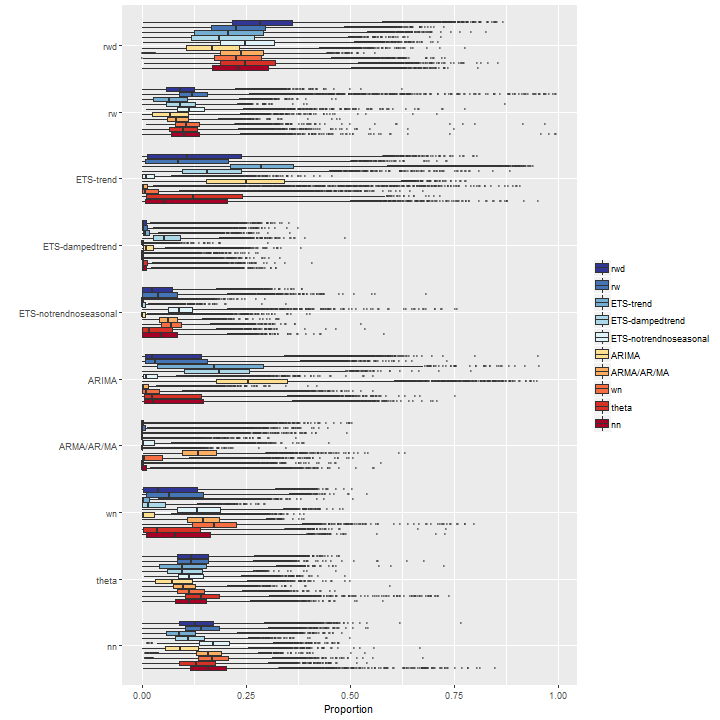
\includegraphics{figures/yearlyoob-1.png}
\caption{\label{fig:yearlyoob}Visualization of the vote matrix based on OOB
sample for yearly random forest. The Y-axis denotes what was predicted
from the random forest. The X-axis denotes the proportion of times each
time series was classified to each class. The colours of boxplots
correspond to class label of the ``best'' forecast-model identified
based on MASE and sMAPE. On each row, distribution of correctly
classified class dominates, indicating a good classification of the
meta-learner.}
\end{figure}

\autoref{fig:viyearly} shows how important each one of the features we
considered within each class as well as in the overall classification
mechanism of the FFORMS.

According to \autoref{fig:viyearly}, the features related to strength of
trend, nonstationarity (ur\_pp, diff1y\_acf1), overall shape of the
trend (linear: measured by linearity, damped trend: measured by beta,
exponential: measured by curvature) and measures of randomness (from
spikiness, and lmres\_acf1) are the most important for the choice of
yearly time series forecast-models. The first ACF value of the original
series (y\_acf1) appears among the top five within the random walk with
drift class and the ARMA/AR/MA class as it helps to separate stationary
and non-stationary series. The first correlation coefficient of the
twice-differenced series is appeared to be the most important in the
ARIMA class as this class contains the higher order differenced series.
The Hurst exponent and entropy appear to be equally important in
stationary classes. Within the ETS-damped trend class beta and curvature
ranked as important features. The length of time series (N) is assigned
relatively high rank within the random walk with drift, ETS-dampedtrend
and the neural-network class compared to others. On the other hand, sum
of squares of the first five autocorrelation coefficients of the
twice-difference series and the lumpiness are the least important
feature across many classes.

\autoref{fig:pdpyearly} shows the partial dependency curves, and the
associated confidence intervals of the top-three features that get
selected most in each class. The three features show a non-linear
relationship with the predicted class probabilities. The probabilities
of selecting ETS-trend, ARIMA, ETS-without seasonal and trend component
and neural network models increase steadily as ur\_pp increases. As
expected, the probability of selecting stationary models decreases as
the test statistic of Phillip-Perron test increases and this probability
remains zero beyond the value of 0 of ur\_pp.~Random walk with drift,
ETS-trend, ETS-damped trend, ARIMA show an increasing relationship with
trend, whereas the random walk, ETS-without trend and seasonal
components, and the stationary models show a monotonically deceasing
relationship as trend increases. The theta class shows parabolic
relationship with trend. It is interesting to observe that the
probability of selecting neural network models decreases with very high
trend value. The reason could be very clear highly trended series are
more likely to select ETS-trend, ETS-dampedtrend and ARIMA models. The
wide confidence bands around the partial dependency functions of
linearity indicate the higher variability of ICE curves. The probability
of selecting random walk with drift increases rapidly beyond value 0 and
remains thereafter. The PDP curves of linearity in ARMA/AR/MA increase
sharply around 0 and decline steadily after that. Similar relationship
can be observed within the white noise class with wide confidence bands
whereas ARIMA and neural network show the opposite relationship. The
partial dependency curves of diff1y\_acf1 indicate the probabilities of
selecting the random walk with drift and the ETS-trend are higher for
differenced-stationary series.

\autoref{fig:friedmany} shows the heat maps of the relative strength of
all possible pairwise interactions of the features for each class. The
relative strength of two-way interactions between features are measured
using the formula developed by \textcite{friedman2008predictive}, which
is implemented in the \texttt{iml} (\textcite{molnar2018iml},) package
in R. Except the ETS-trend class, trend and ur\_pp show a high level of
interactivity and a less interactivity with other features. Linearity
also show a weak interaction with other features in all classes. In
almost all the classes the partial correlation and auto-correlation
based features are heavily interacting. However, the first correlation
coefficient of the differenced series does not interact with other
features heavily within the ARIMA class. Further, almost all pairs of
features appear to be interacting within neural network category. The
interactivity between stability and lumpiness is the most common type of
interactivity appear within all classes.

\begin{figure}
\centering
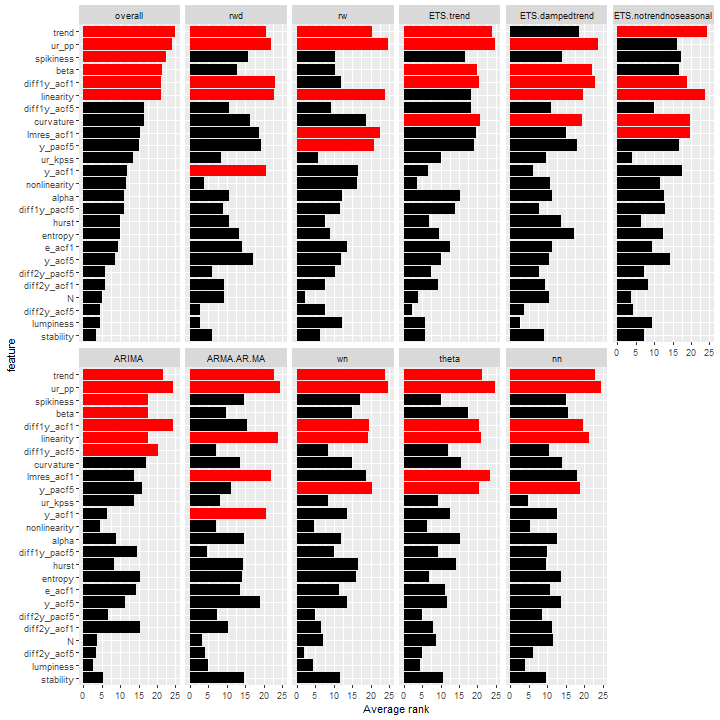
\includegraphics{figures/viyearly-1.pdf}
\caption{\label{fig:viyearly}Feature importance plot for yearly series.
Overall feature importance(top left plot) is evaluated based on two
measures: i) Permutation-based variable importance measure and ii) mean
decrease in Gini coefficients are used to evaluate shown in the top left
plot. Class-specific feature importance is evaluated based on three
measures: i) permutation-based variable importance, PD-based variable
importance measure, and ICE-based variable importance measure. Longer
bars indicate more important features. Top 5 overall features are
highlighted in purple. Strength of trend appears to be the most
important feature.}
\end{figure}

\newpage

\begin{figure}
\centering
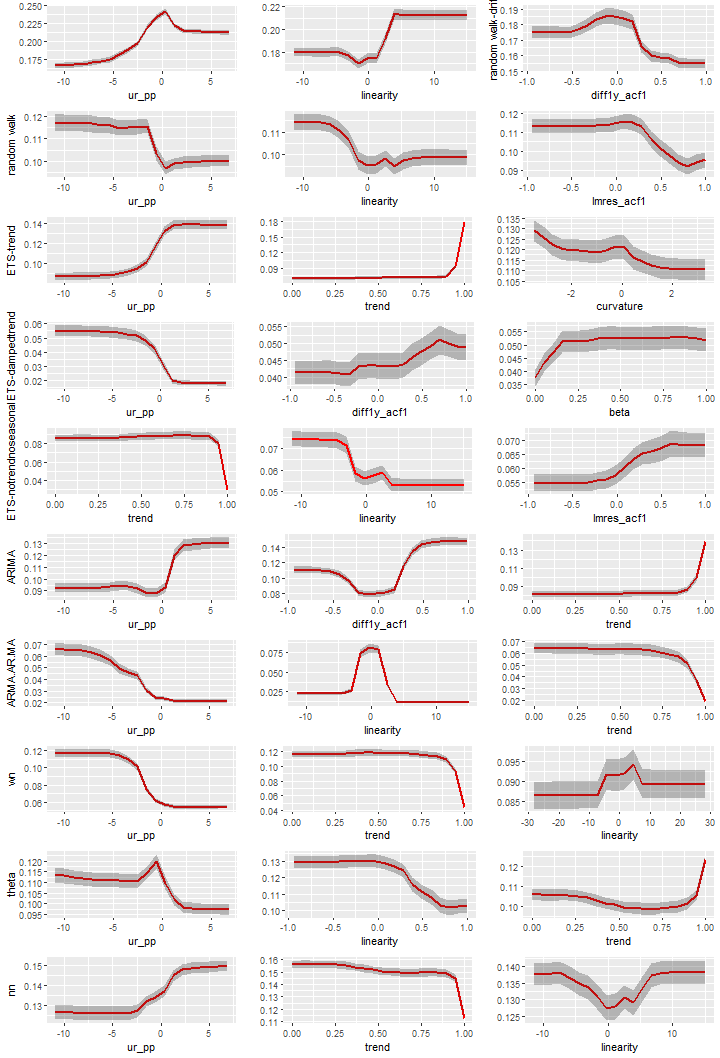
\includegraphics{figures/pdpyearly-1.png}
\caption{\label{fig:pdpyearly}Partial dependence plots for the top-three
features get selected most within each class for yearly series. The
shading shows the 95\% confidence intervals. Y-axis denotes the
probability of belong to corresponding class. All features show a
nonlinear relationship with predicted probabilities.}
\end{figure}

\newpage

\begin{figure}
\centering
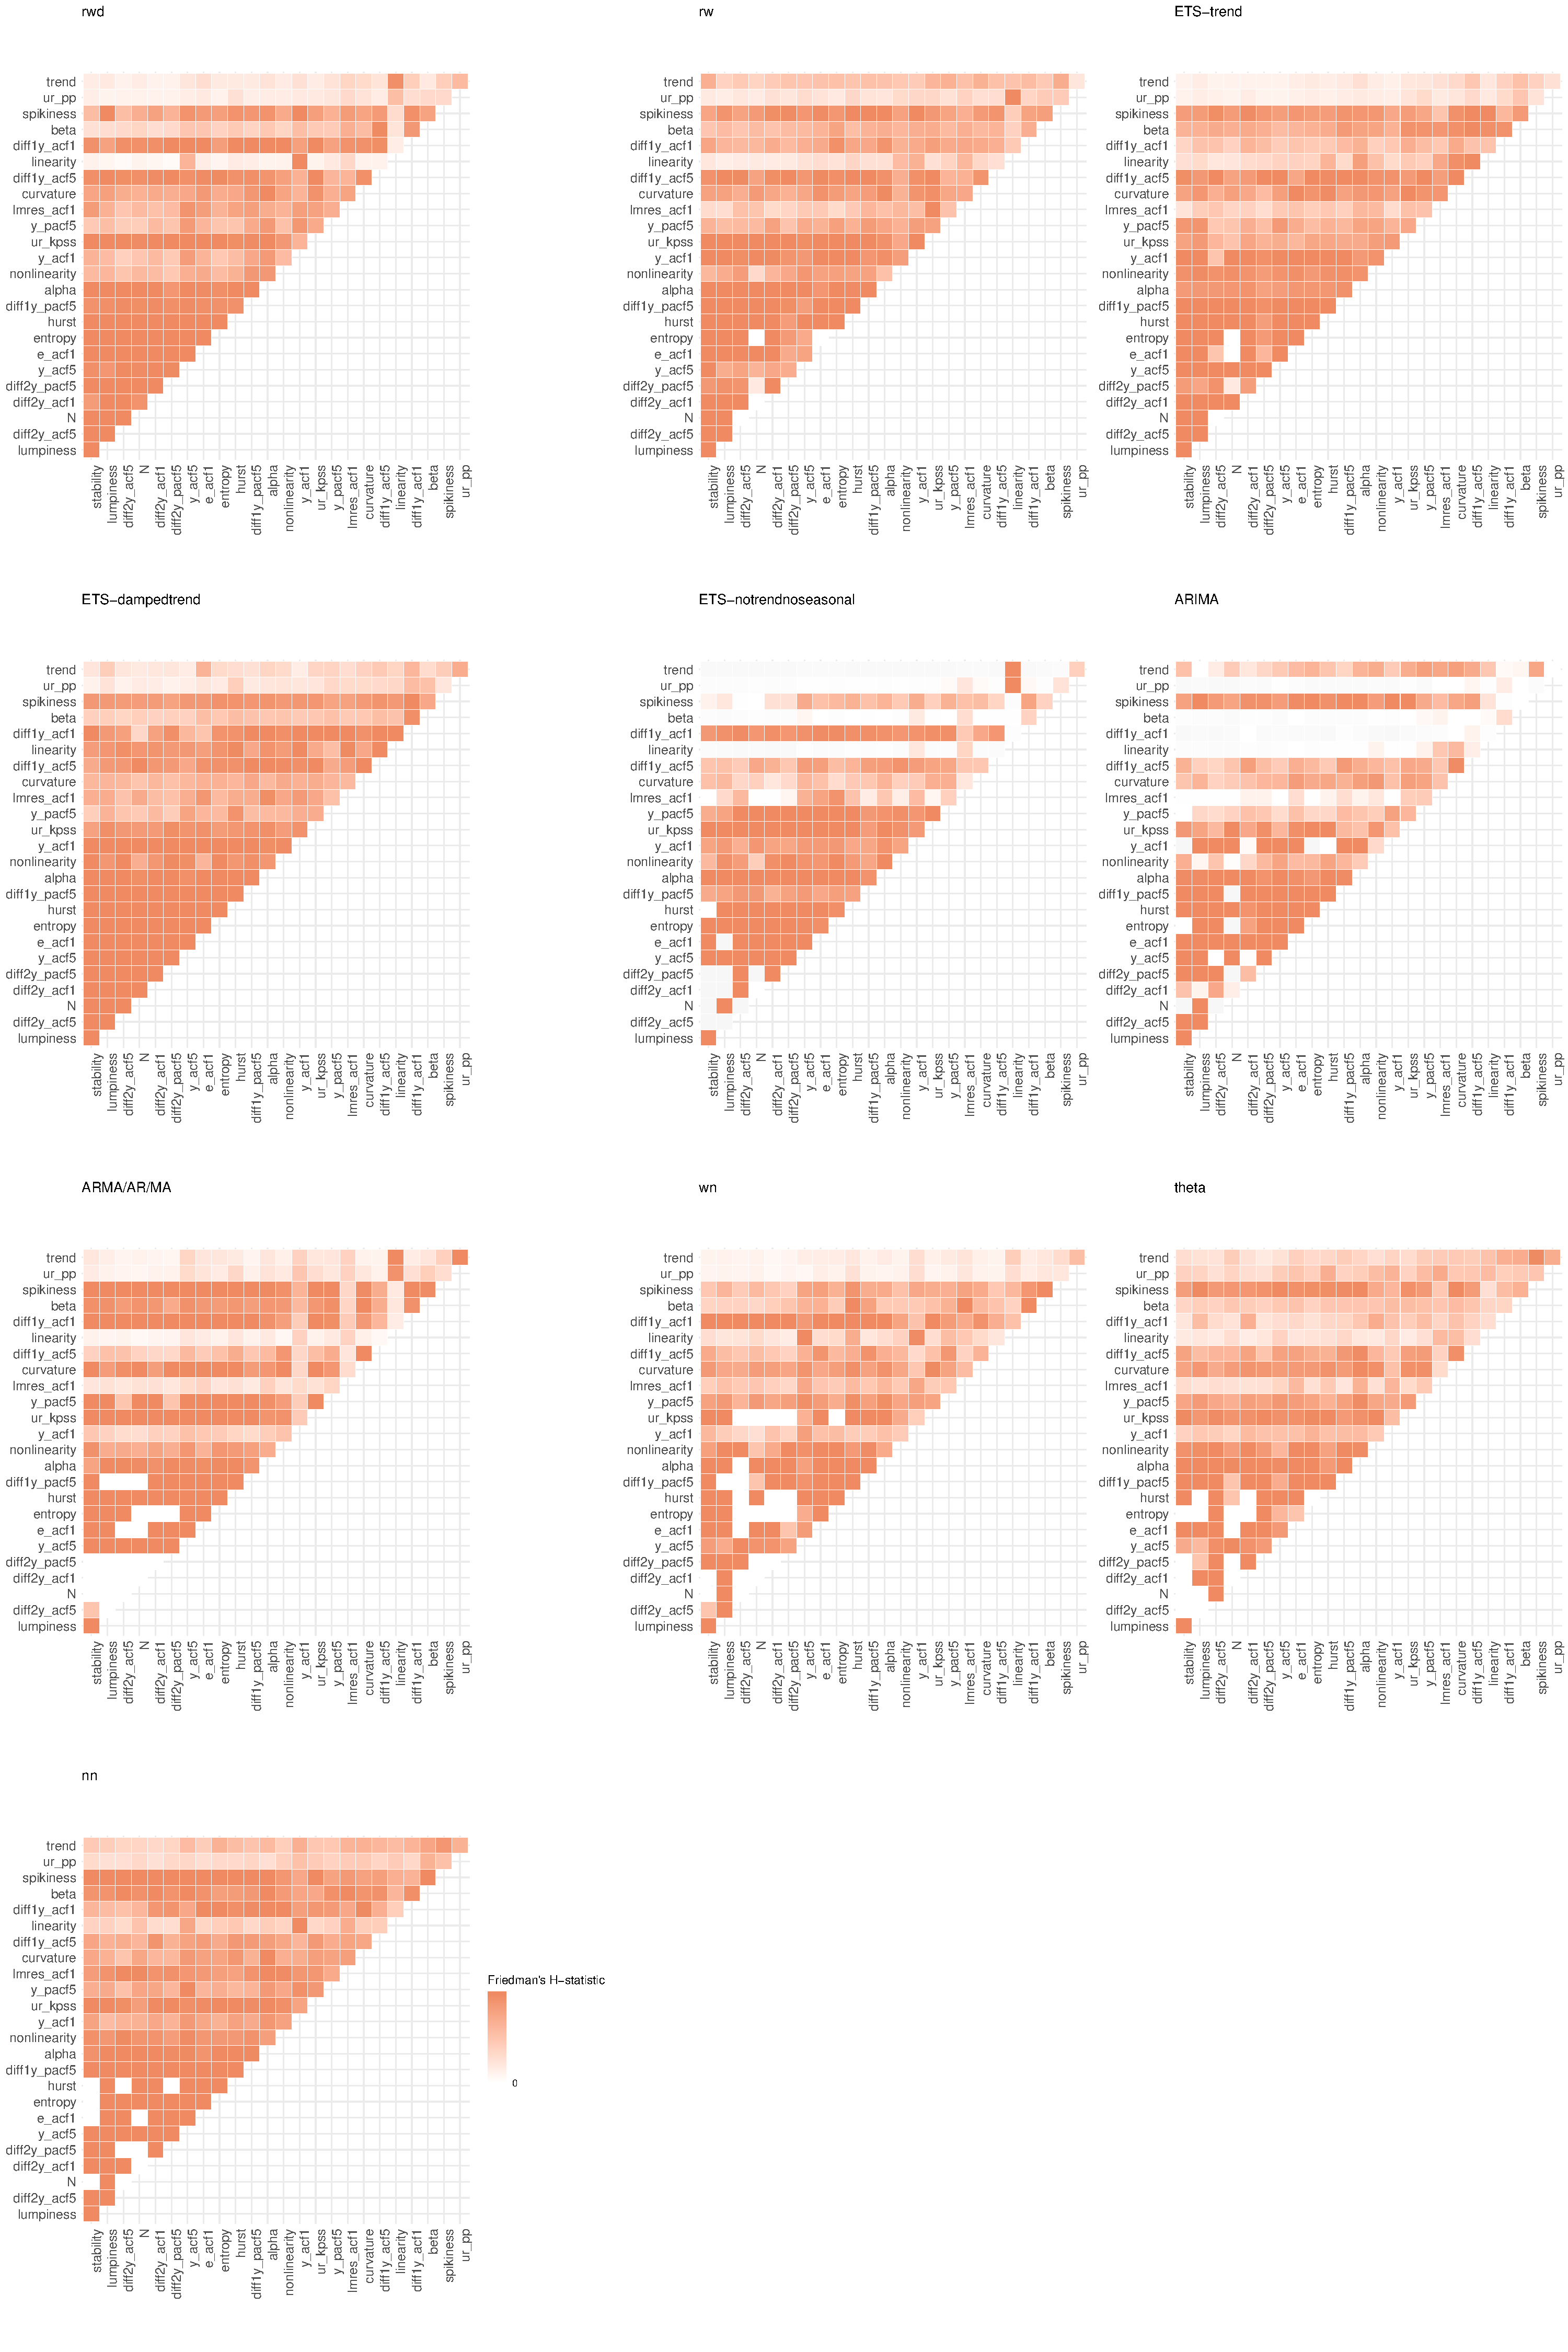
\includegraphics{figures/friedmany-1.pdf}
\caption{\label{fig:friedmany}Heat maps of relative strength of all possible
pairwise interactions calculated based on Friedman's H-statistic (yearly
series). Strength of trend shows less interactivity with other
features.}
\end{figure}

\newpage

\subsection{Quarterly and Monthly
data}\label{quarterly-and-monthly-data}

\autoref{fig:oobquarterlymonthly1} - \autoref{fig:oobquarterlymonthly2}
show the vote-matrices of the random forests for quarterly and monthly
data respectively based on OOB observations.
\autoref{fig:oobquarterlymonthly1} and
\autoref{fig:oobquarterlymonthly2} depicted similar patterns across
classes. For quarterly and monthly data, the same set of features and
the class-labels are used to train the model. Hence, this consistency
between the results of the quarterly and the monthly series would
provide evidence in support of the validity and trustability of the
model. The outliers associated with the dominating distributions
indicate some series are correctly classified with very high
probability. Seasonal time series have a low chance of classified into
the random walk with drift model and a high chance of selecting SARIMA,
stlar and tbats. Except the time series labelled as ARMA/AR/MA all other
quarterly time series have a very low chance of classified into
ARMA/AR/MA class. Further, all distributions correspond to the tbats row
located further away from zero. This indicates all-time series select
tbats model at least once from the individual trees in the forest.
Except few outliers, distributions within neural network category also
show a slight upward deviation from the zero. However, the upper
boundaries of these distributions do not surpass the upper boundaries of
dominating box plots in the random walk with drift class and the SARIMA
class. Further, within stlar, tbats, theta and neural network classes
all distributions level at similar proportionalities. These types of
similarities in the distributions indicate the appropriateness of using
combination forecasting. Further, these information is useful in
identifying potential time series models for combination forecast and
improve the existing combination approaches proposed in the
M4-competition (\textcite{Makridakis2018dx}). In addition to that the
similarities and diversities observed in the boxplots indicate the
neighbourhood of cases in their respective instance space.

\autoref{fig:viquarterly} and \autoref{fig:vimonthly} show feature
importance plots for the quarterly and monthly data respectively. For
both quarterly and monthly data strength of seasonality, trend,
linearity and spikiness are the most important features across all
categories. Even though the lumpiness does not appear as a top five
feature within classes it is appeared to be an important feature in the
overall classification process and a relatively high ranks are assigned
within many classes. In the case of yearly data low variable importance
is assigned to both stability and length of the series. However, within
quarterly and monthly data a high variable importance is assigned to
length of the series and stability. One notable difference between the
quarterly series and the monthly series is, for monthly data length of
the series is ranked among the top five, specially in random walk with
drift, random walk, ETS with seasonal and trend component, ETS-seasonal,
SARIMA and ARIMA classes. In addition to the strength of seasonality,
the models handling seasonal components (snaive, SARIMA, all ETS models
with seasonal component) assigned a high importance to the additional
features related to seasonality such as ACF, PACF-based features related
to seasonal lag or seasonally differenced series. Furthermore, as
expected features calculated based on parameter estimated of ETS(A, A,
A) ranked as important for the choice of ETS with damped trend and
seasonal component and ETS with trend and seasonal component.

\autoref{fig:pdpquarterly1} and \autoref{fig:pdpquarterly2} show the
partial dependency functions of the features that get selected most
often in the top. Additionally, the PDP of N is included to observe the
effects stated in the literature \autocite{makridakis2000m3}. Except for
random walk, partial dependency curves of seasonality and trend show a
similar behaviour for both quarterly and monthly data. Hence, for
seasonality and trend, the partial dependency curves computed based
quarterly are presented except for random walk. Probability of selecting
a model with a parameter to handle the seasonal effect (snaive, all ETS
models with seasonal component, SARIMA, tbats, theta, stlar) increases
as the seasonality increases. Further, the rwd, all ETS model with trend
component, SARIMA, ARIMA, tbats and theta, have a high probability of
getting selected as the strength of trend increases. On the other hand,
opposite relationships are observed for snaive and ETS-seasonal. This
confirms the idea that the choice of model selection consistent with the
expected relationships. For quarterly series the probability of
selecting random walk models remains stable up to 0.85 value of trend
and drops sharply afterwards, whereas the FFORMS framework for monthly
series show probability of selecting random walk models increases as
trend increases. This could be due to the interaction effect of trend
with other features.

\autoref{fig:friedmanQ} and \autoref{fig:friedmanM} show the heat maps
of the relative strength of all possible pairwise interactions
calculated based on Friedman's H-statistic for quarterly and monthly
data respectively. Within the random walk with drift class trend shows a
high interactivity with other features. Within all classes seasonality
show less interactivity with other features, whereas lumpiness shows
high interactivity with other features. Further within each class, a
subset of ACF/PACF-based features show some interactivity. In general
interactivity between features related to correlation structure of a
time series and overall shape (spikiness, linearity, curvature, etc)
lead to the choice of forecast-model selection.

\begin{figure}
\centering
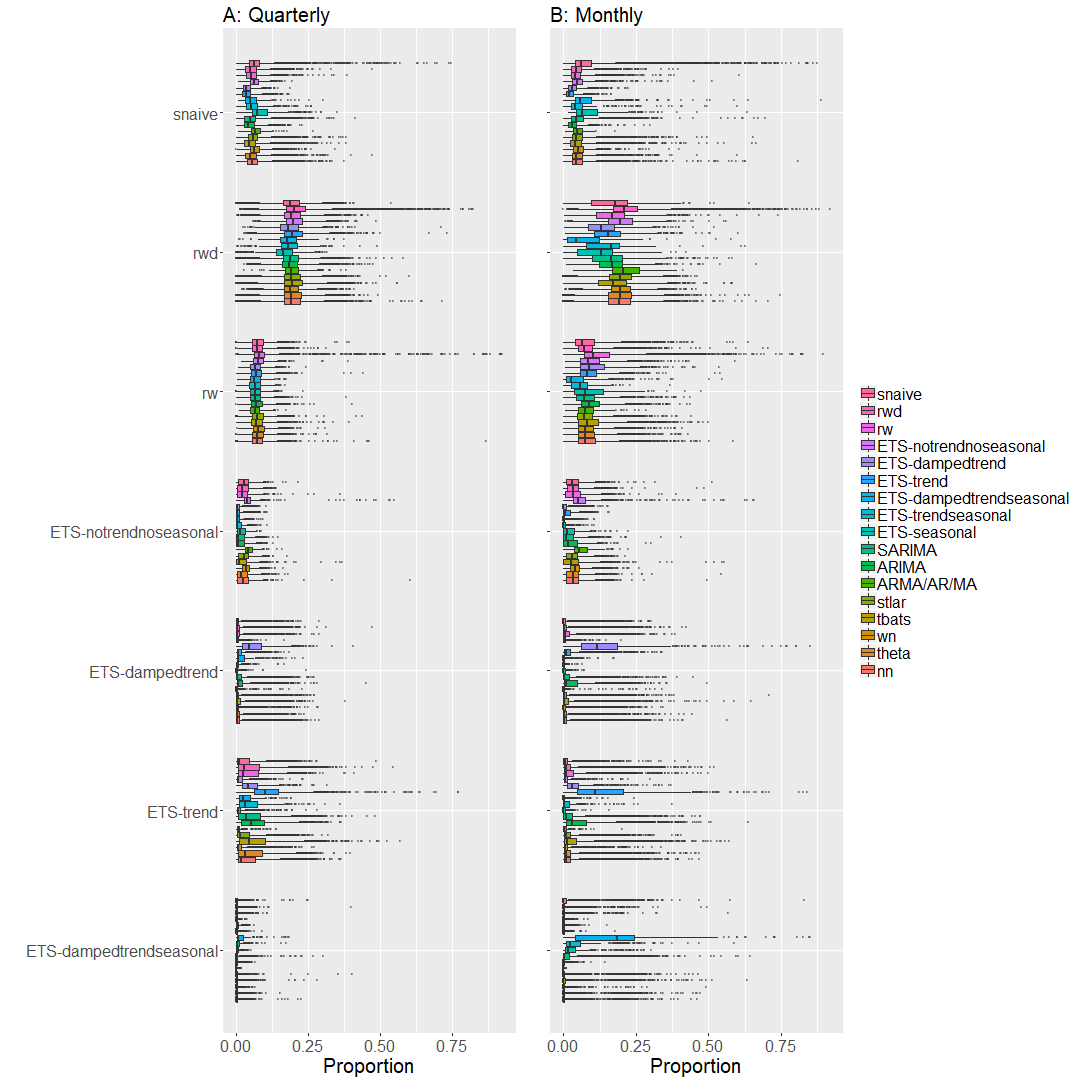
\includegraphics{figures/oobquarterlymonthly1-1.png}
\caption{\label{fig:oobquarterlymonthly1}Visualization of the vote matrix
based on OOB sample for quarterly random forest. The Y-axis denotes what
was predicted from the random forest?. The X-axis denotes the proportion
of times each time series was classified to each class. The colours of
boxplots corresponds to class label of the ``best'' forecast-model
identified based on MASE and sMAPE. On each row, distribution of
correctly classified class dominates, indicating a good classification
of the meta-learner. ARMA/AR/MA has a low chance of being selected while
random walk with drift has a high chance of being selected.}
\end{figure}

\clearpage

\begin{figure}
\centering
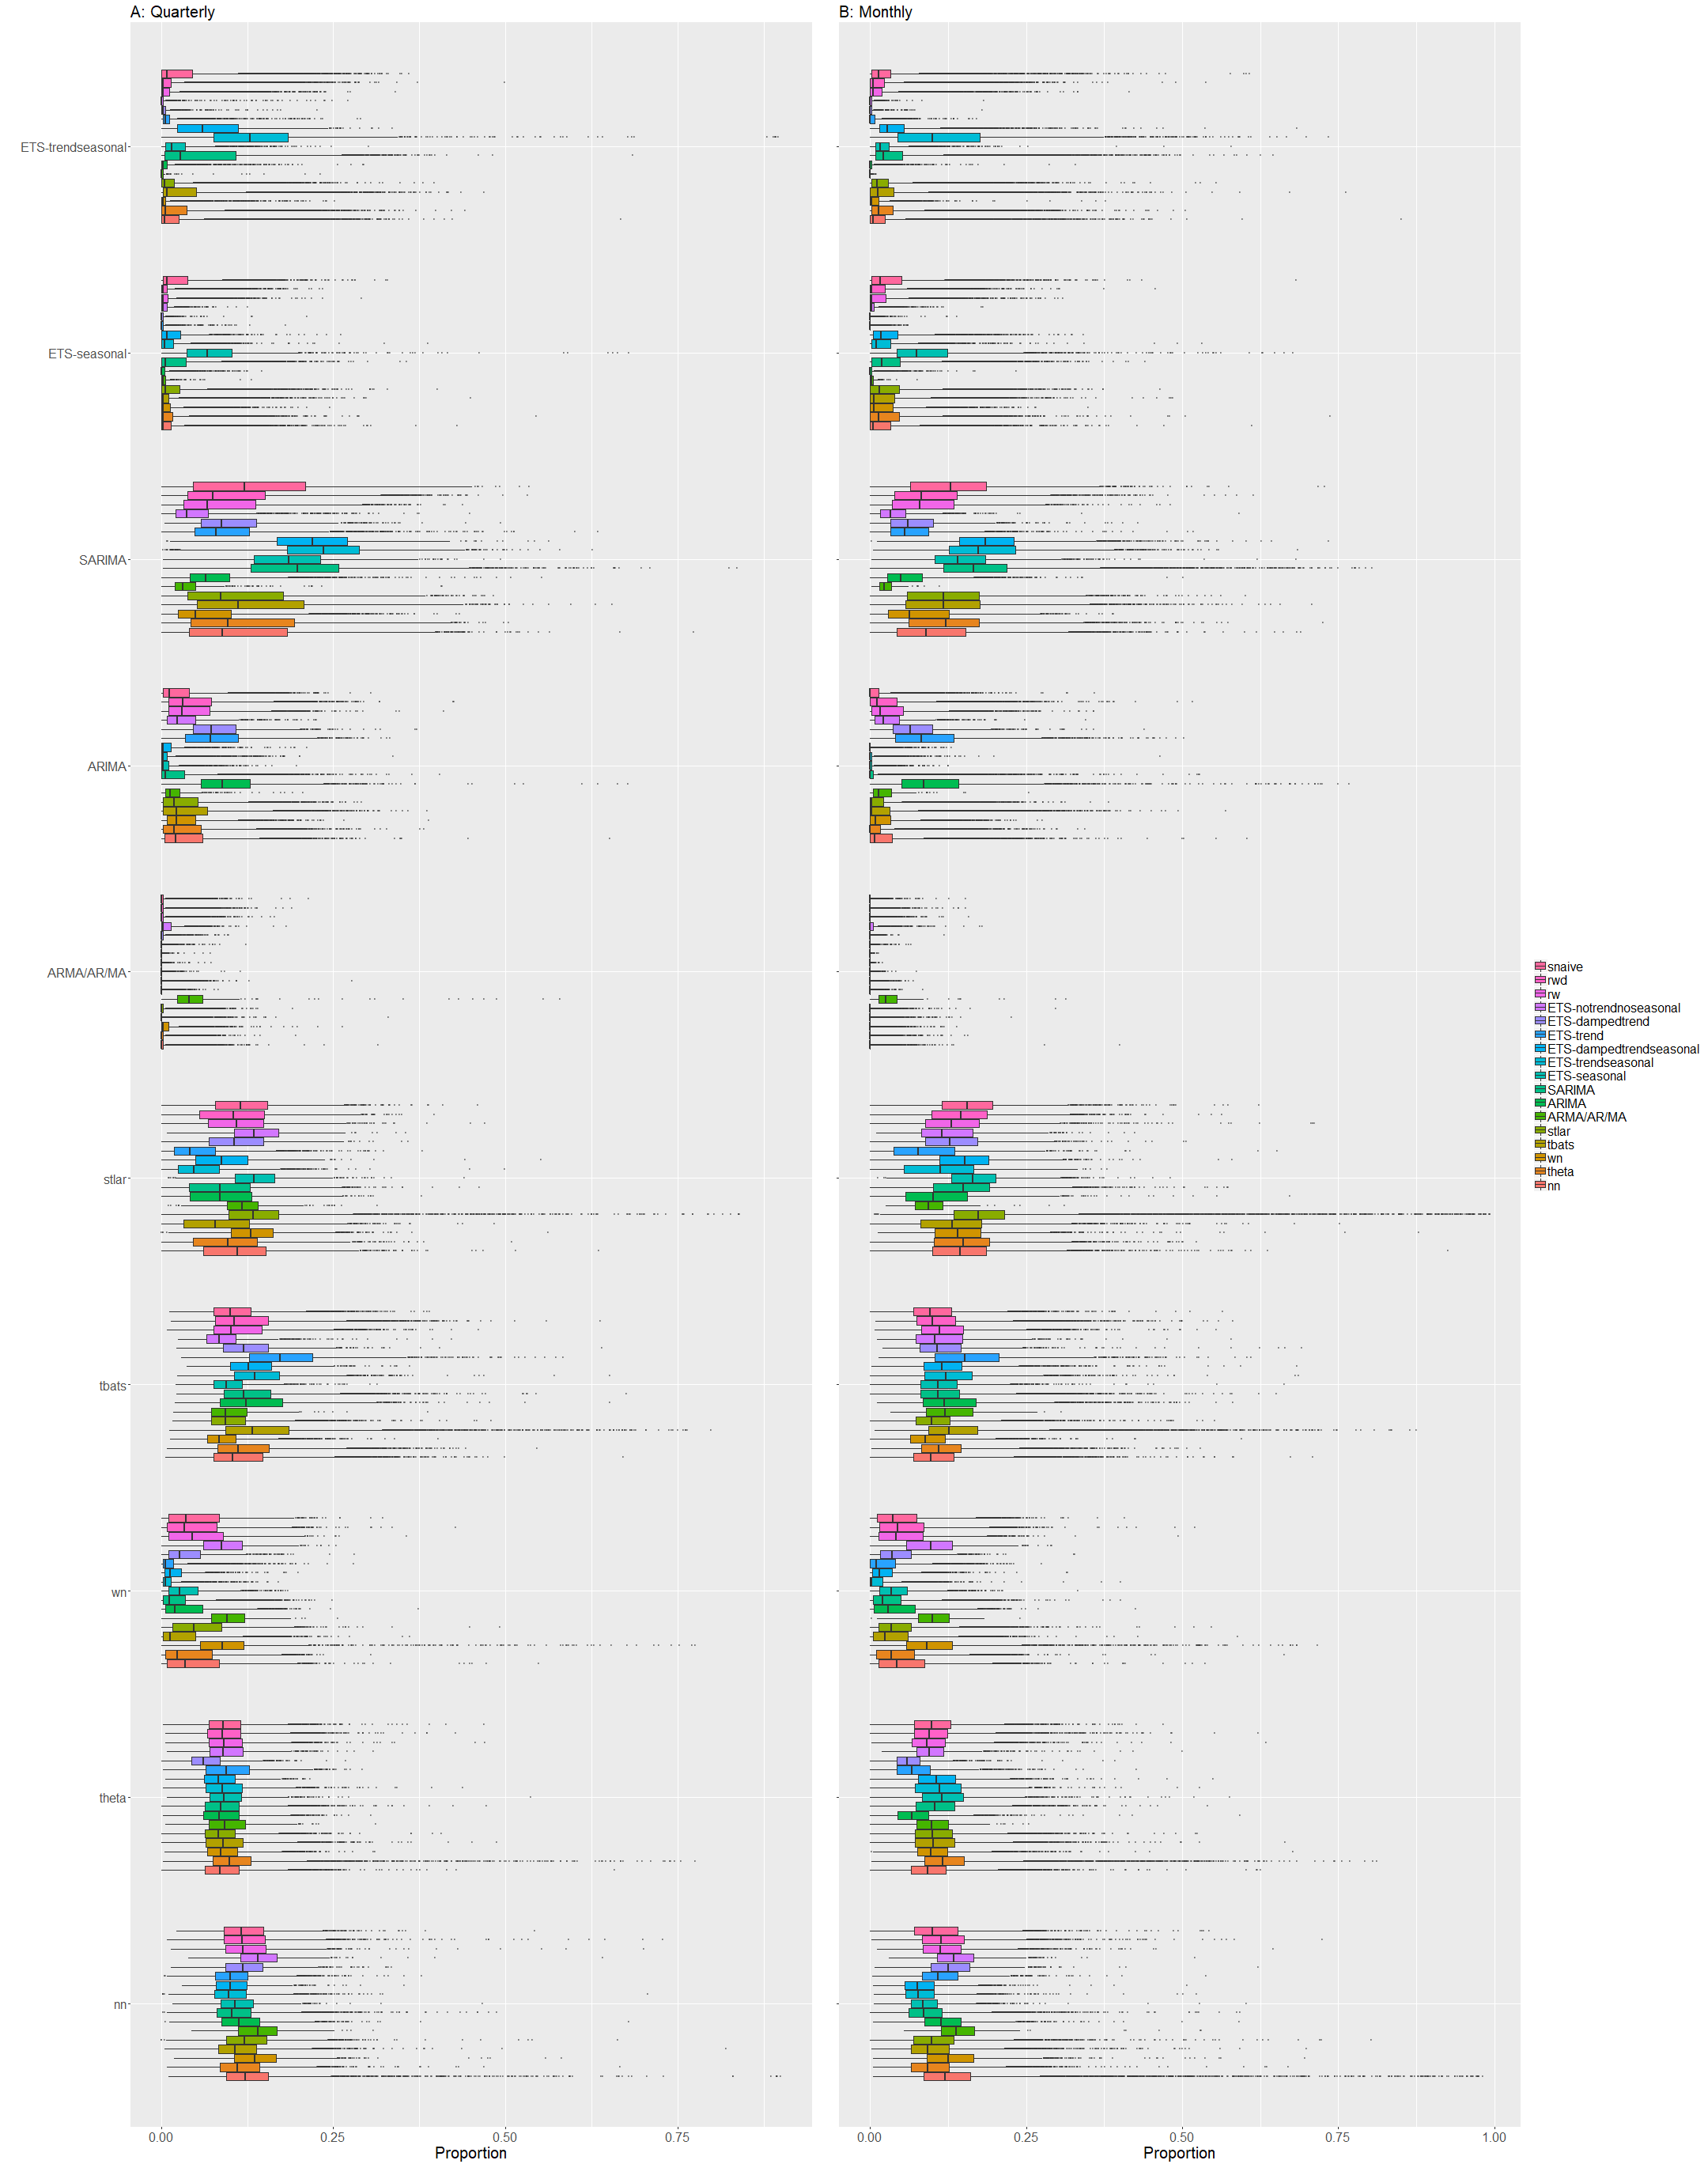
\includegraphics{figures/oobquarterlymonthly2-1.png}
\caption{\label{fig:oobquarterlymonthly2} Visualization of the vote matrix
based on OOB sample for monthly random forest. The Y-axis denotes what
was predicted from the random forest? The X-axis denotes the proportion
of times each time series was classified to each class. The colours of
boxplots corresponds to class label of the ``best'' forecast-model
identified based on MASE and sMAPE. On each row, distribution of
correctly classified class dominates, indicating a good classification
of the meta-learner. Few series correspond to stlar and nn have been
correctly classified with a very high probability.}
\end{figure}

\clearpage

\begin{figure}[h]

{\centering 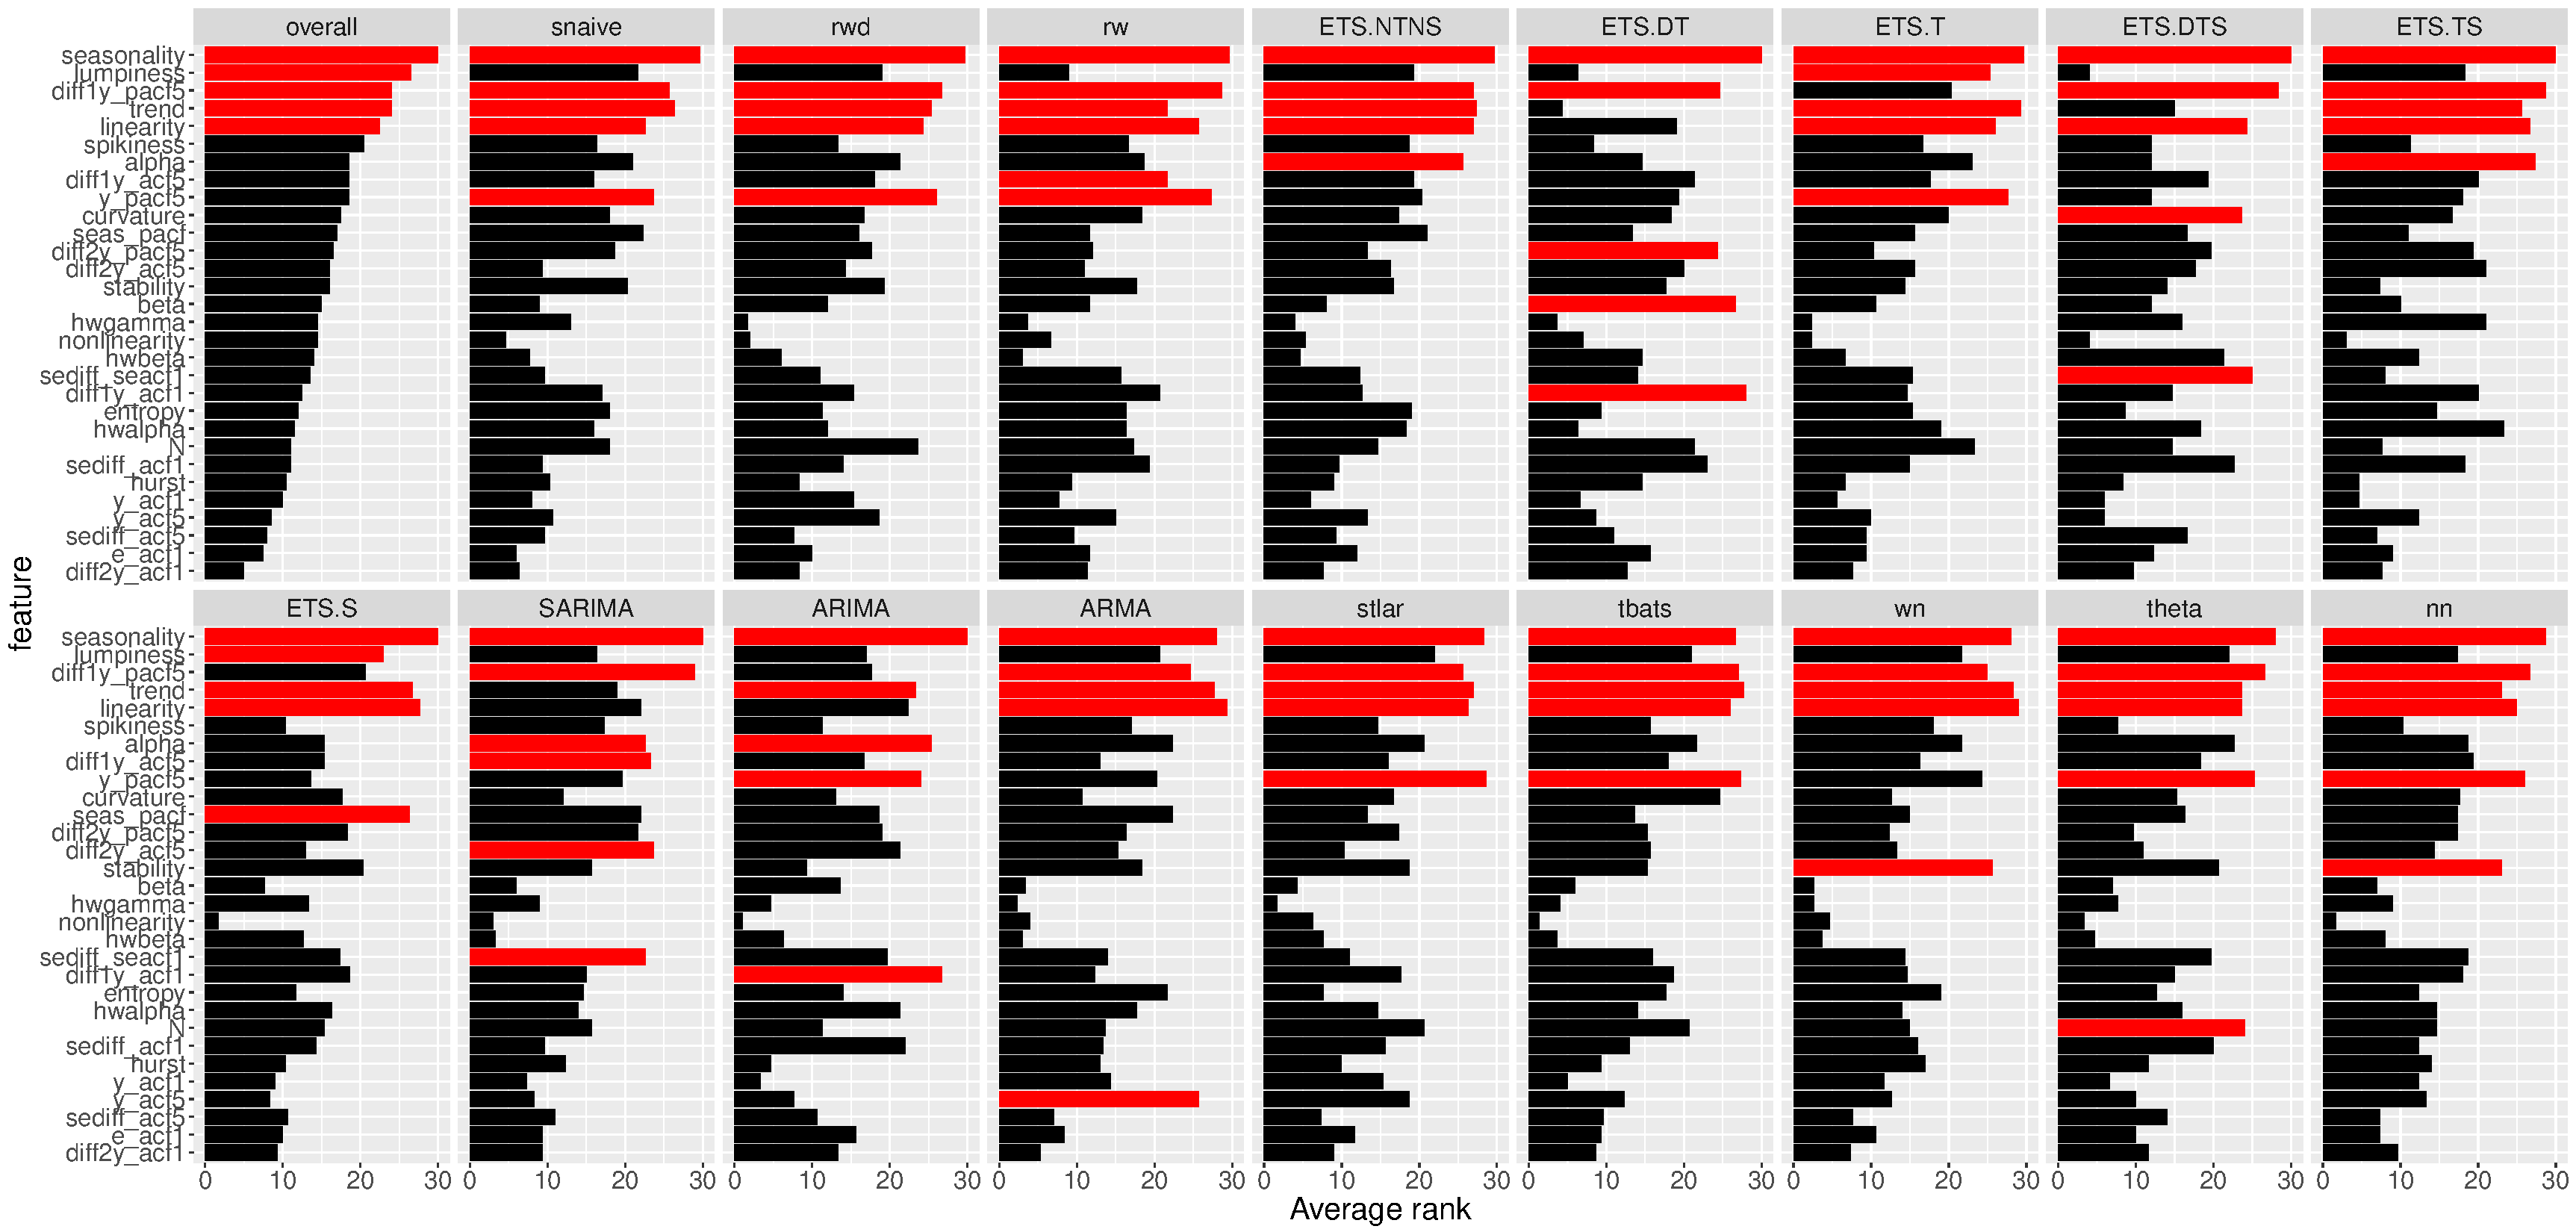
\includegraphics{figures/viquarterly-1} 

}

\caption{Feature importance plot for quarterly data. Permutation-based VI measure and mean decrease in Gini coefficients are used to evaluate overall feature importance. Class-specific feature importance is evaluated based on the three measures: permutation-based VI, PD-based VI measure, and ICE-based VI measure. Longer bars indicate more important features. Top 5 features are highlighted in red.}\label{fig:viquarterly}
\end{figure}

\begin{figure}[h]

{\centering 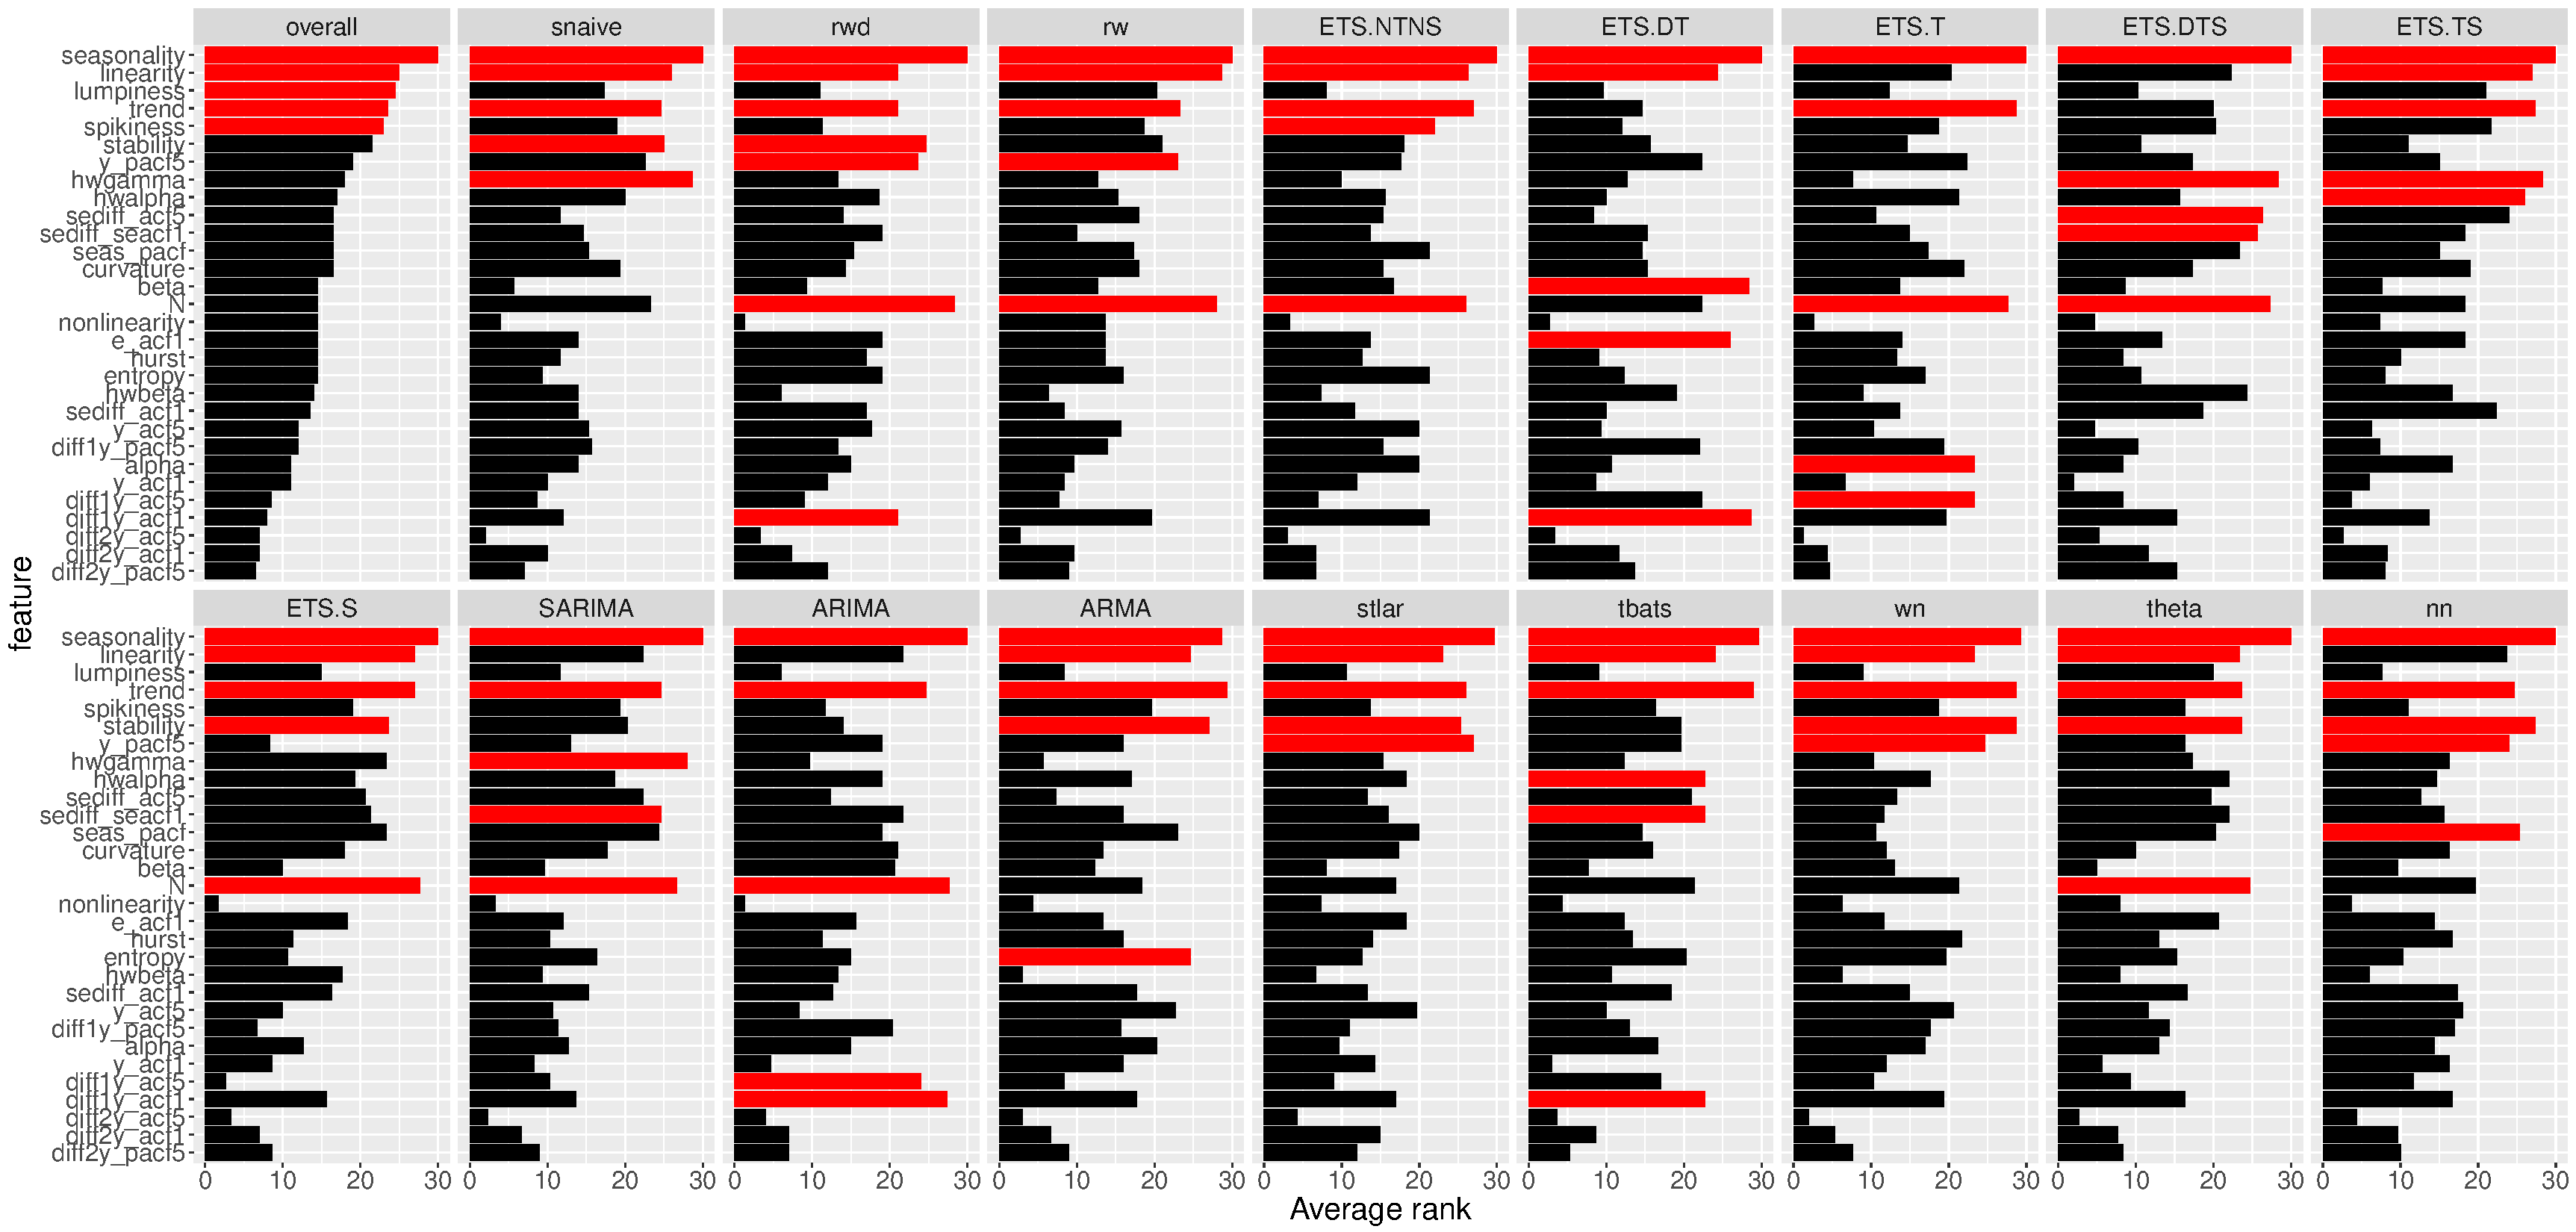
\includegraphics{figures/vimonthly-1} 

}

\caption{Feature importance plot for monthly data. Permutation-based VI measure and mean decrease in Gini coefficients are used to evaluate overall feature importance. Class-specific feature importance is evaluated based on the three measures: permutation-based VI, PD-based VI measure, and ICE-based VI measure. Longer bars indicate more important features. Top 5 features are highlighted in red.}\label{fig:vimonthly}
\end{figure}

\newpage

\begin{figure}
\centering
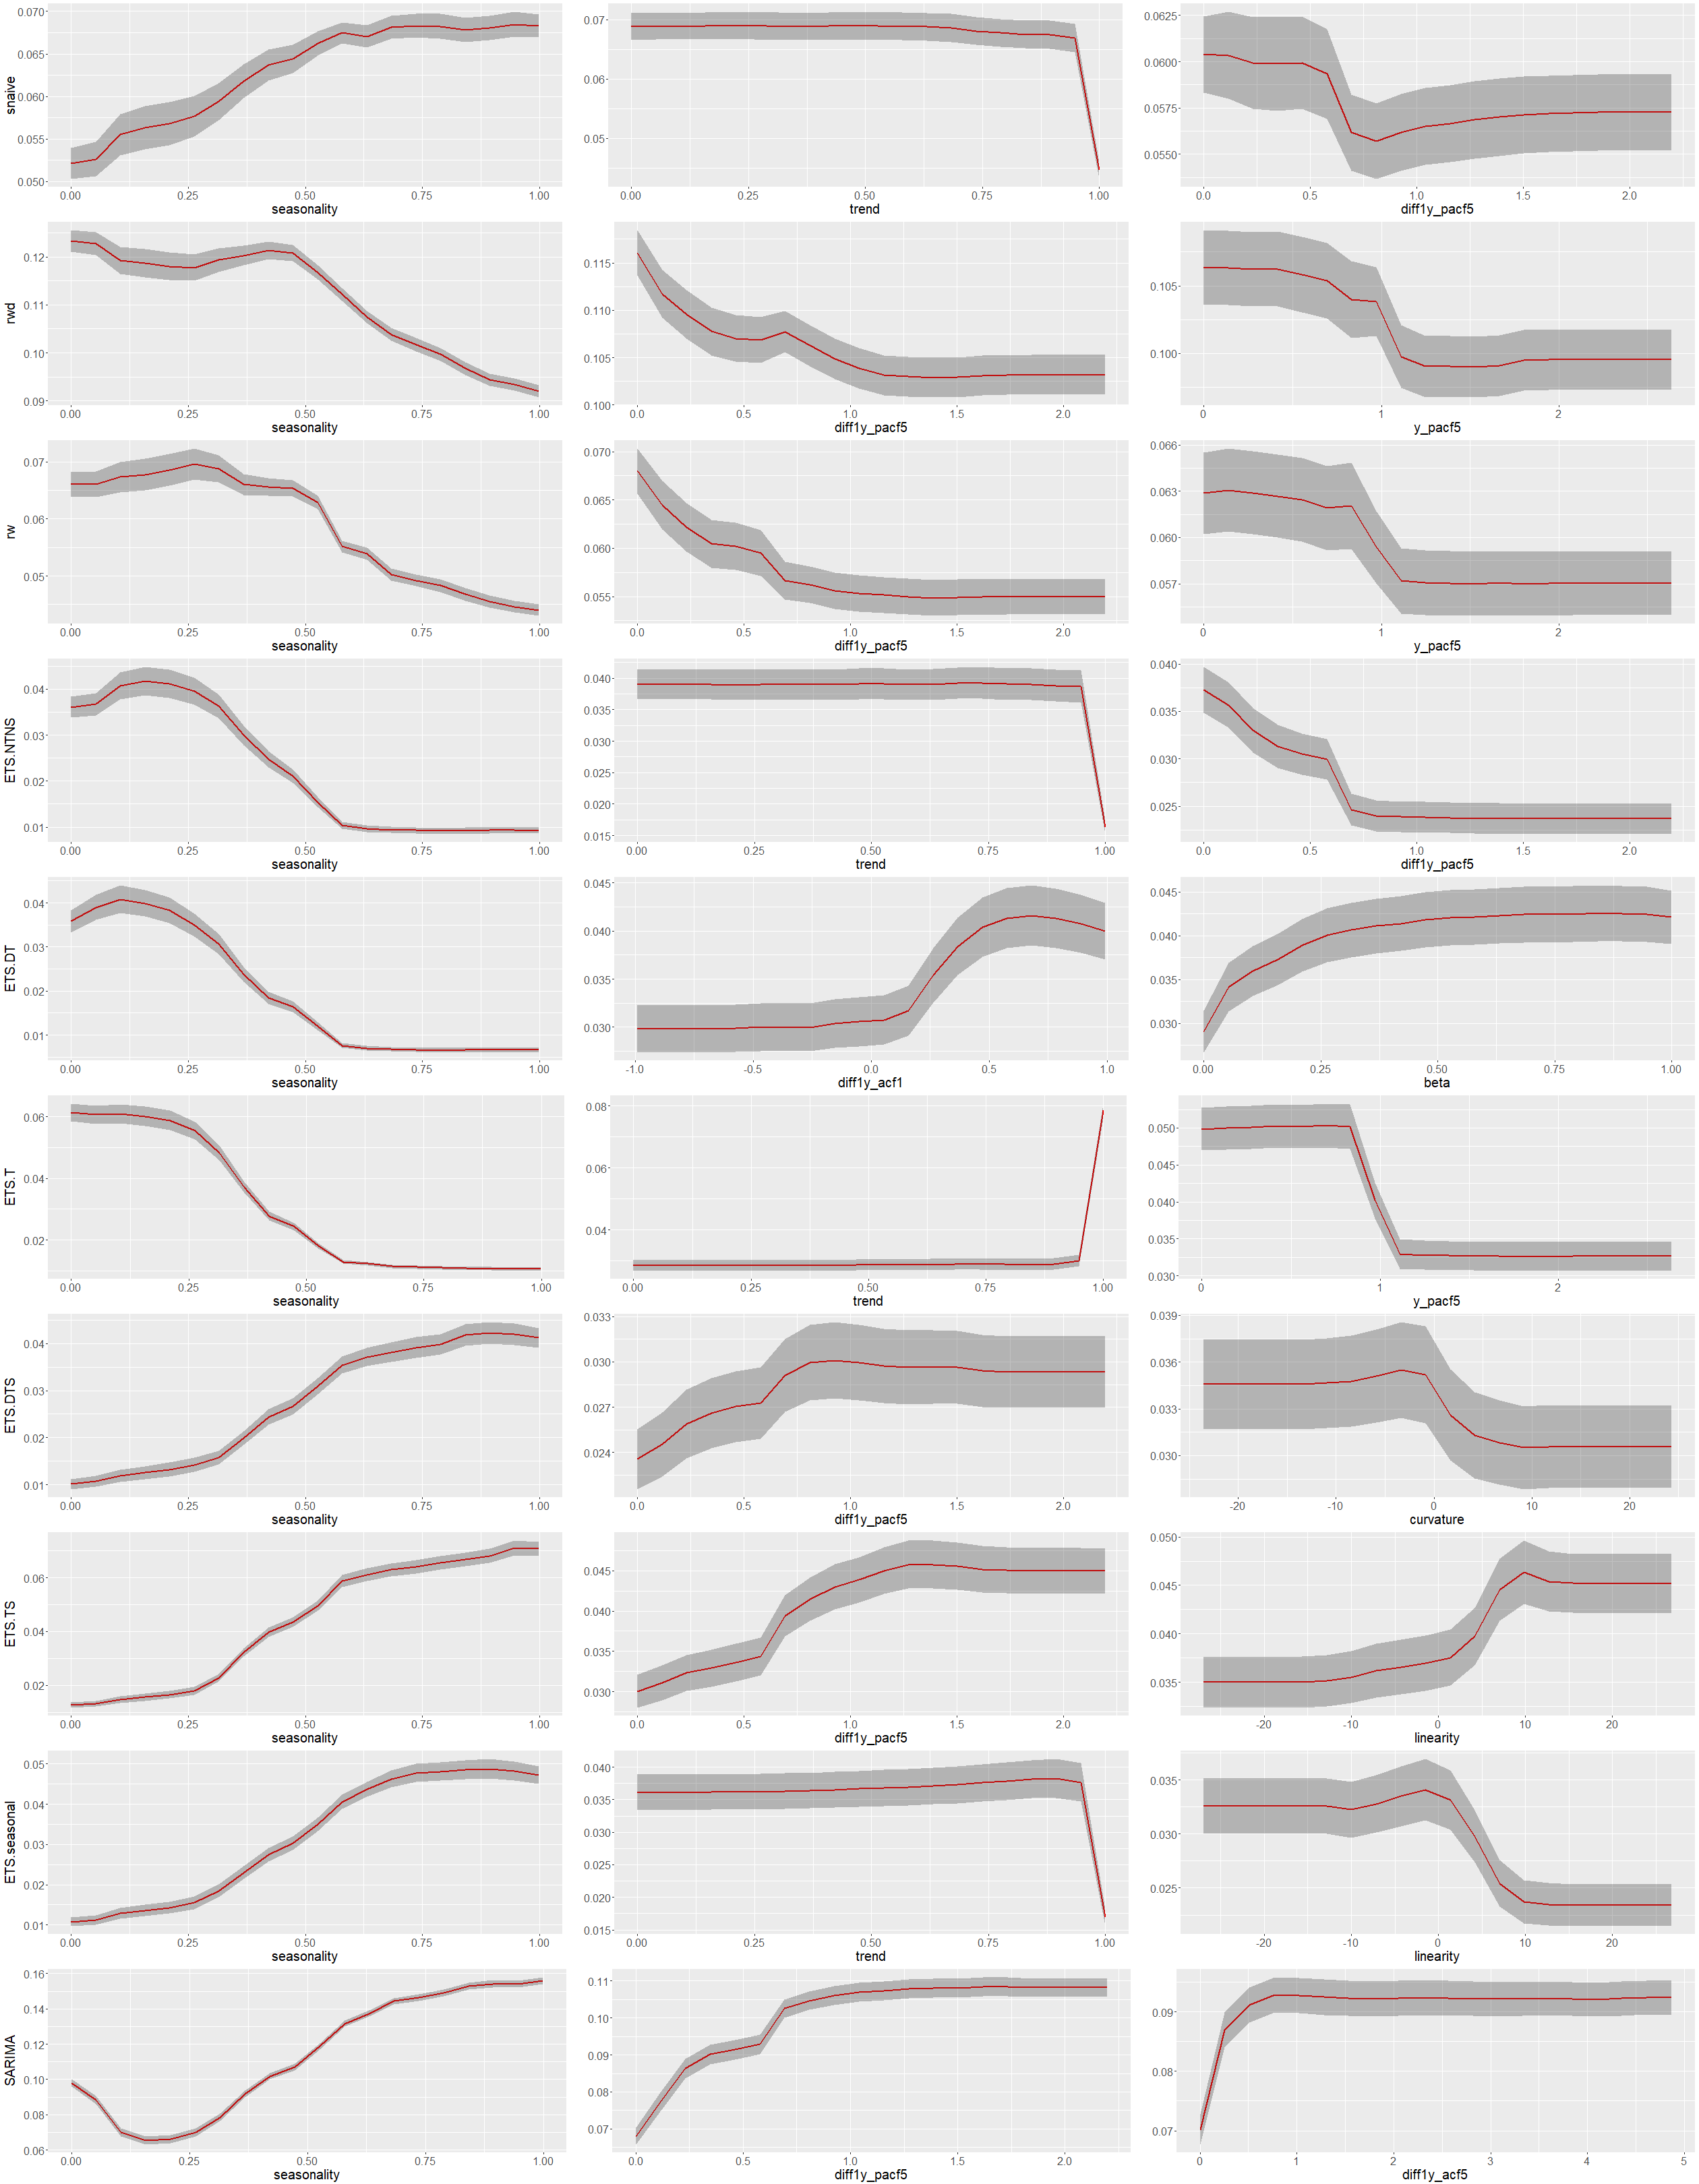
\includegraphics{figures/pdpquarterly1-1.png}
\caption{\label{fig:pdpquarterly1}Partial dependence plots for the top-three
features get selected most within each class inside quarterly and
monthly FFORMS frameworks. Additionally, N is included to observe the
effects stated in the literature. The shading shows the 95\% confidence
interval. Y-axis denotes the probability of belonging to corresponding
class. Red colour is for PDP drawn based on quarterly data and blue
colour is for the PDP drawn based on monthly data.}
\end{figure}

\newpage

\begin{figure}
\centering
\includegraphics{figures/pdpquarterlysec2-1.png}
\caption{\label{fig:pdpquarterlysec2}Partial dependence plots for the
top-three features get selected most within each class inside quarterly
and monthly FFORMS frameworks. Additionally, N is included to observe
the effects stated in the literature. The shading shows the 95\%
confidence interval. Y-axis denotes the probability of belonging to
corresponding class. Red colour is for PDP drawn based on quarterly data
and blue colour is for the PDP drawn based on monthly data.(Continue
from Figure 9)}
\end{figure}

\clearpage

\begin{figure}
\centering
\includegraphics{figures/friedmanQM-1.pdf}
\caption{\label{fig:friedmanQM}Heat maps of relative strength of all
possible pairwise interactions calculated based on Friedman's
H-statistic for quarterly and monthly data.}
\end{figure}

\subsection{Weekly}\label{weekly}

\autoref{fig:oobweekly} shows the proportion of times each time series
was classified to each class. Unlike, yearly, quarterly and monthly data
theta method has a low chance of getting selected. The random walk with
drift, tbats models and nn have a high chance of getting selected.
Except ARMA/AR/MA class the distributions corresponds to the true class
label dominate others. ARMA/AR/MA class shows some unusual behaviour
within some categories due to class imbalance ratio, ARMA/AR/MA class
contains fewer number of observations in the training set.

\begin{figure}
\centering
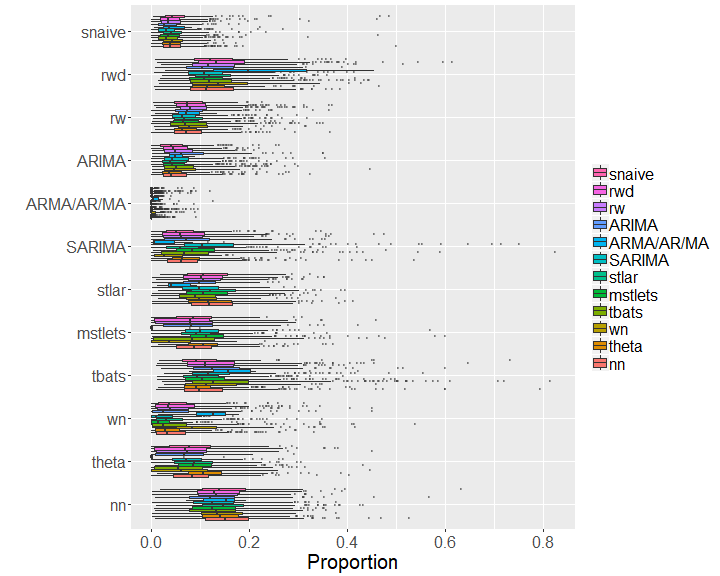
\includegraphics{figures/oobweekly-1.png}
\caption{\label{fig:oobweekly}Visualization of the vote matrix based on OOB
sample for weekly random forest. The Y-axis denotes what was predicted
from the random forest. The X-axis denotes the proportion of times each
time series was classified to each class. The colours of boxplots
corresponds to class label of the ``best'' forecast-model identified
based on MASE and sMAPE. The models rwd, tbats, nn have a high chance of
getting selected.}
\end{figure}

\clearpage

According to the results of \autoref{fig:viweekly} spikiness, linearity,
trend, strength of seasonality, stability and lumpiness have been
assigned a high importance. This is similar to the results of yearly,
quarterly and monthly data. The length of series has been selected among
top 5 by mstlets, tbats, theta and neural network models. According to
the results of \autoref{fig:weeklypdp} for mstlets models probability of
getting selected increases as the linearity increases while the opposite
relationship is observed for SARIMA models. According to
\autoref{fig:weeklypdp} probability of selecting snaive, random walk,
neural network and white noise increases as spikiness increases.
Furthermore, as expected, partial dependency plots reveal probability of
selecting random walk and neural network models decrease as the
stability increases while the opposite relationship can be observed for
white noise class.

\begin{figure}[h]

{\centering 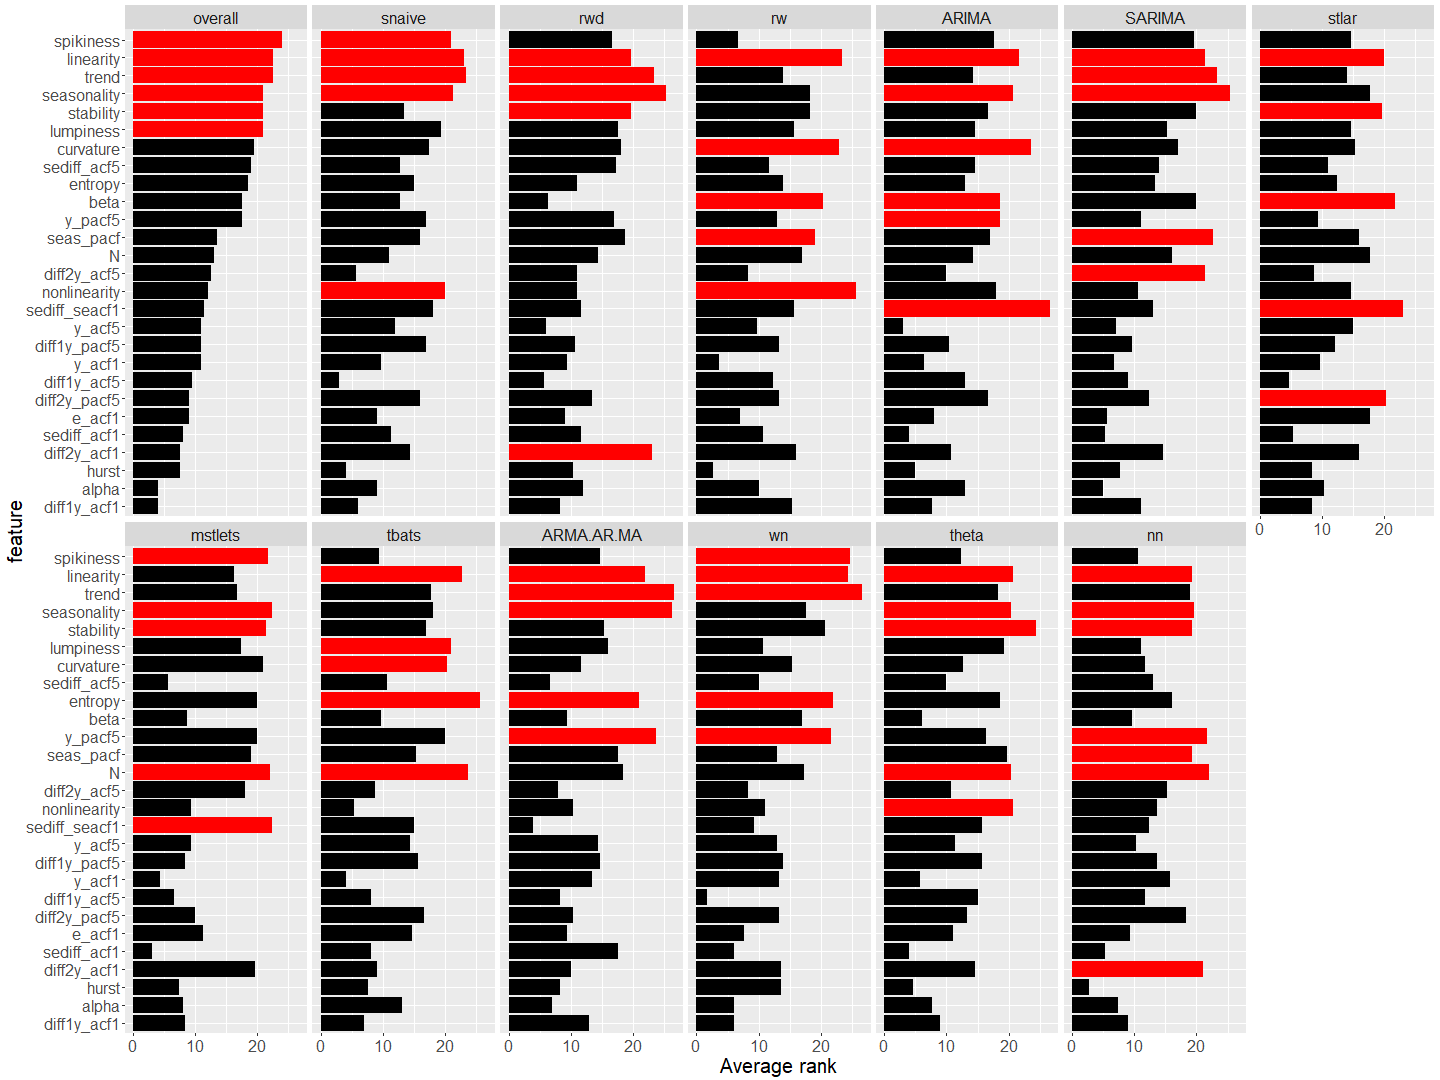
\includegraphics{figures/viweekly-1} 

}

\caption{Feature importance plot for weekly data. Permutation-based VI measure and mean decrease in Gini coefficient is used to evaluate overall feature importance. Class-specific feature importance is evaluated based on the three measures: permutation-based VI, PD-based VI measure, and ICE-based VI measure. Longer bars indicate more important features. Top 5 features are highlighted in red.}\label{fig:viweekly}
\end{figure}

\newpage

\begin{figure}
\centering
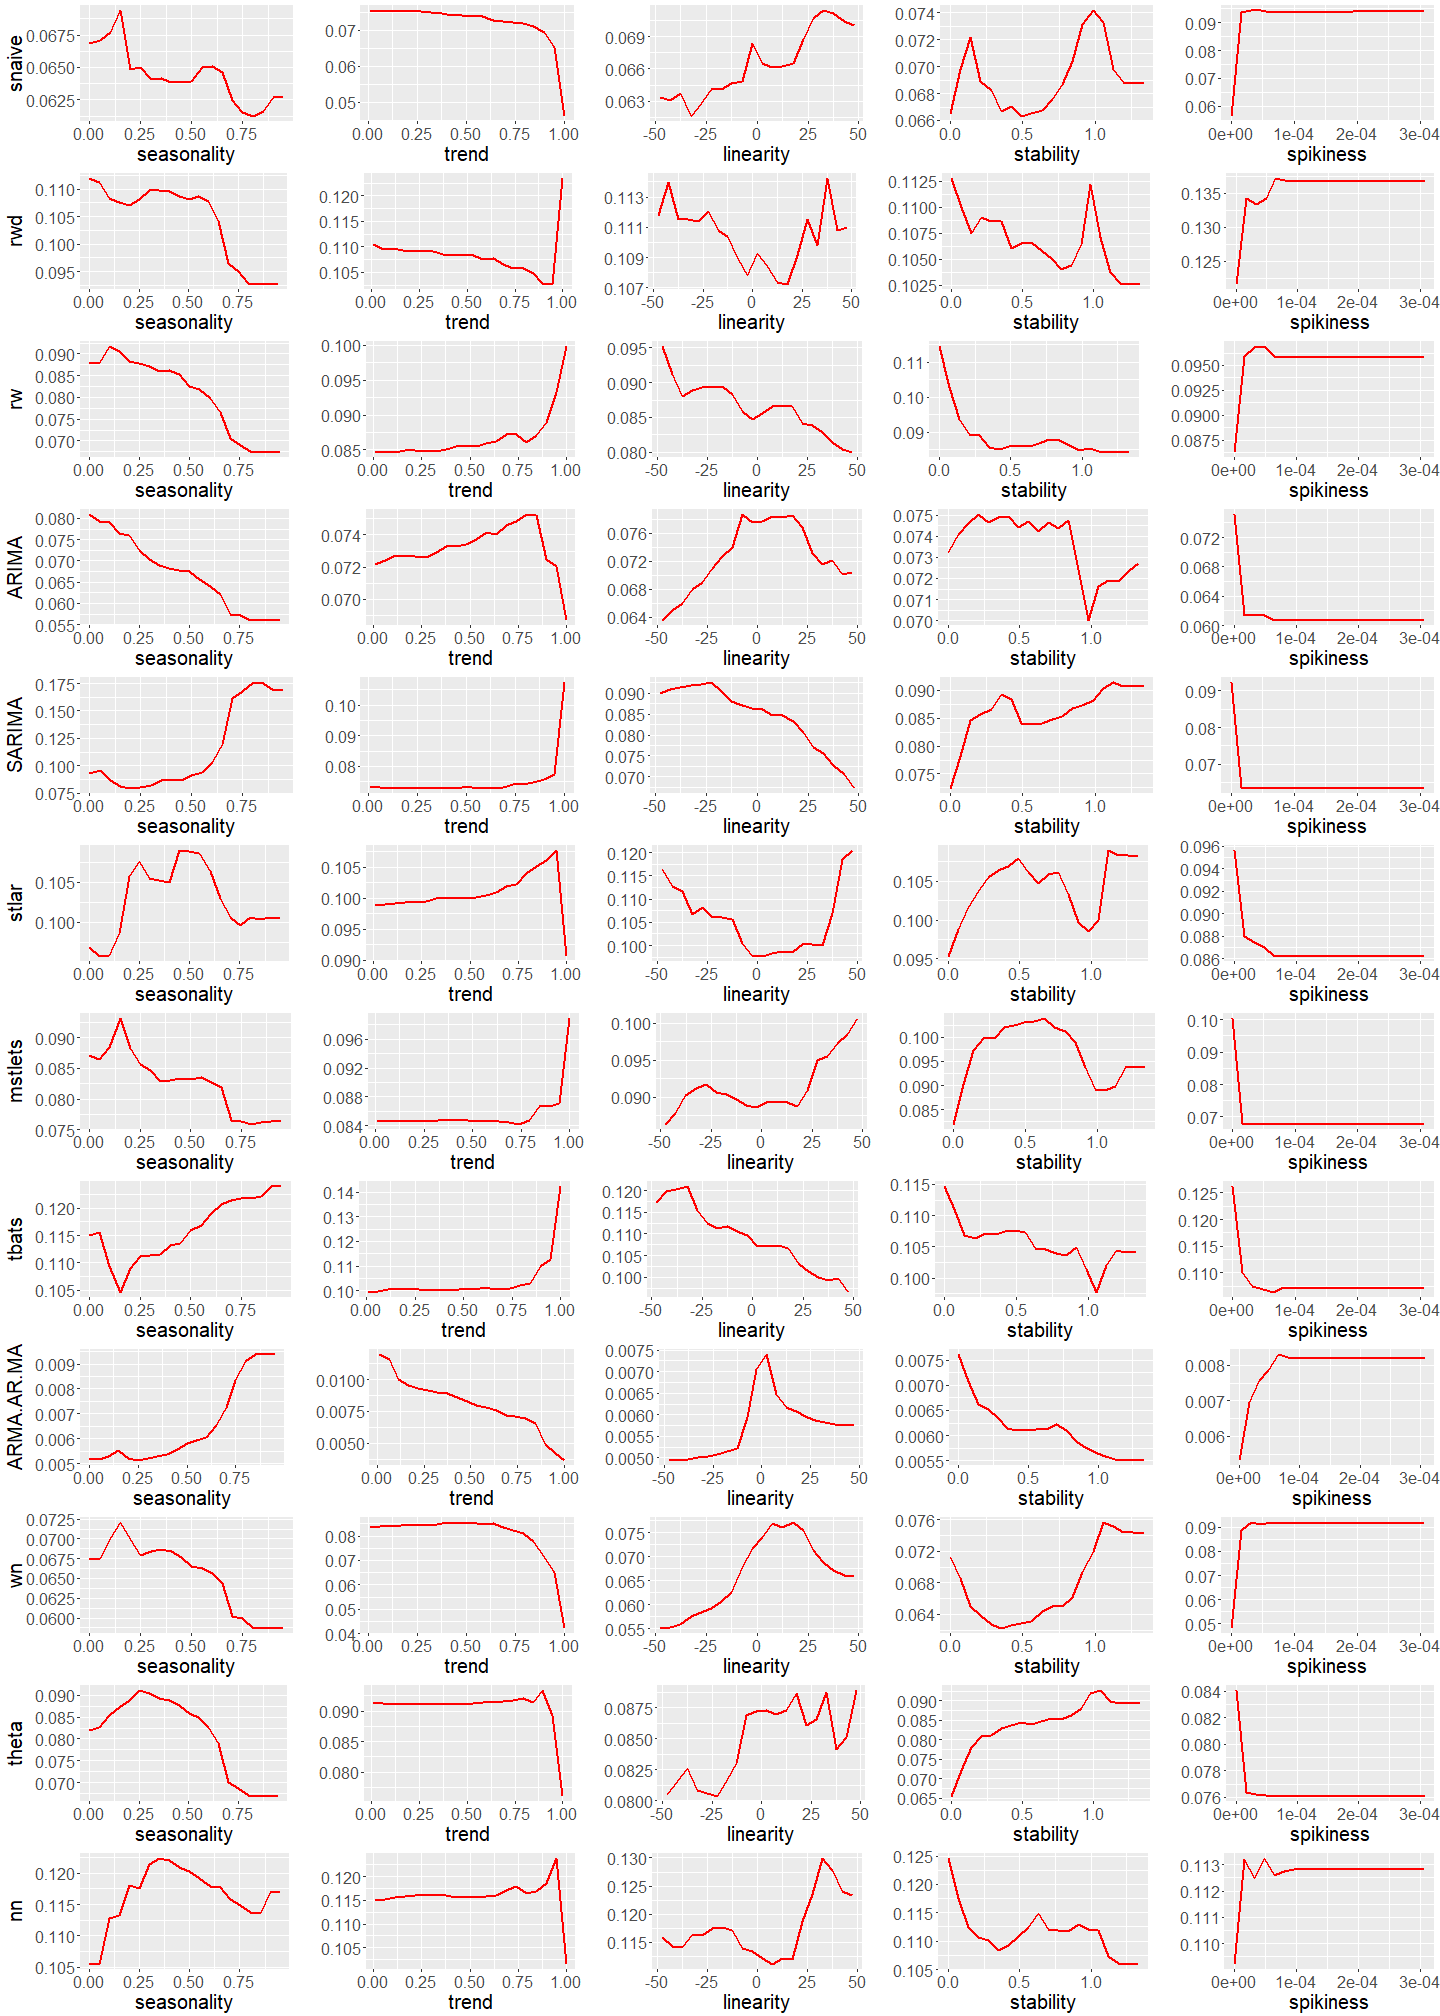
\includegraphics{figures/weeklypdp-1.png}
\caption{\label{fig:weeklypdp}Partial dependence plots for the top ranked
features from variable importance measures (weekly series). The shading
shows the 95\% confidence intervals. Y-axis denotes the probability of
belonging to corresponding class.}
\end{figure}

\newpage

\begin{figure}
\centering
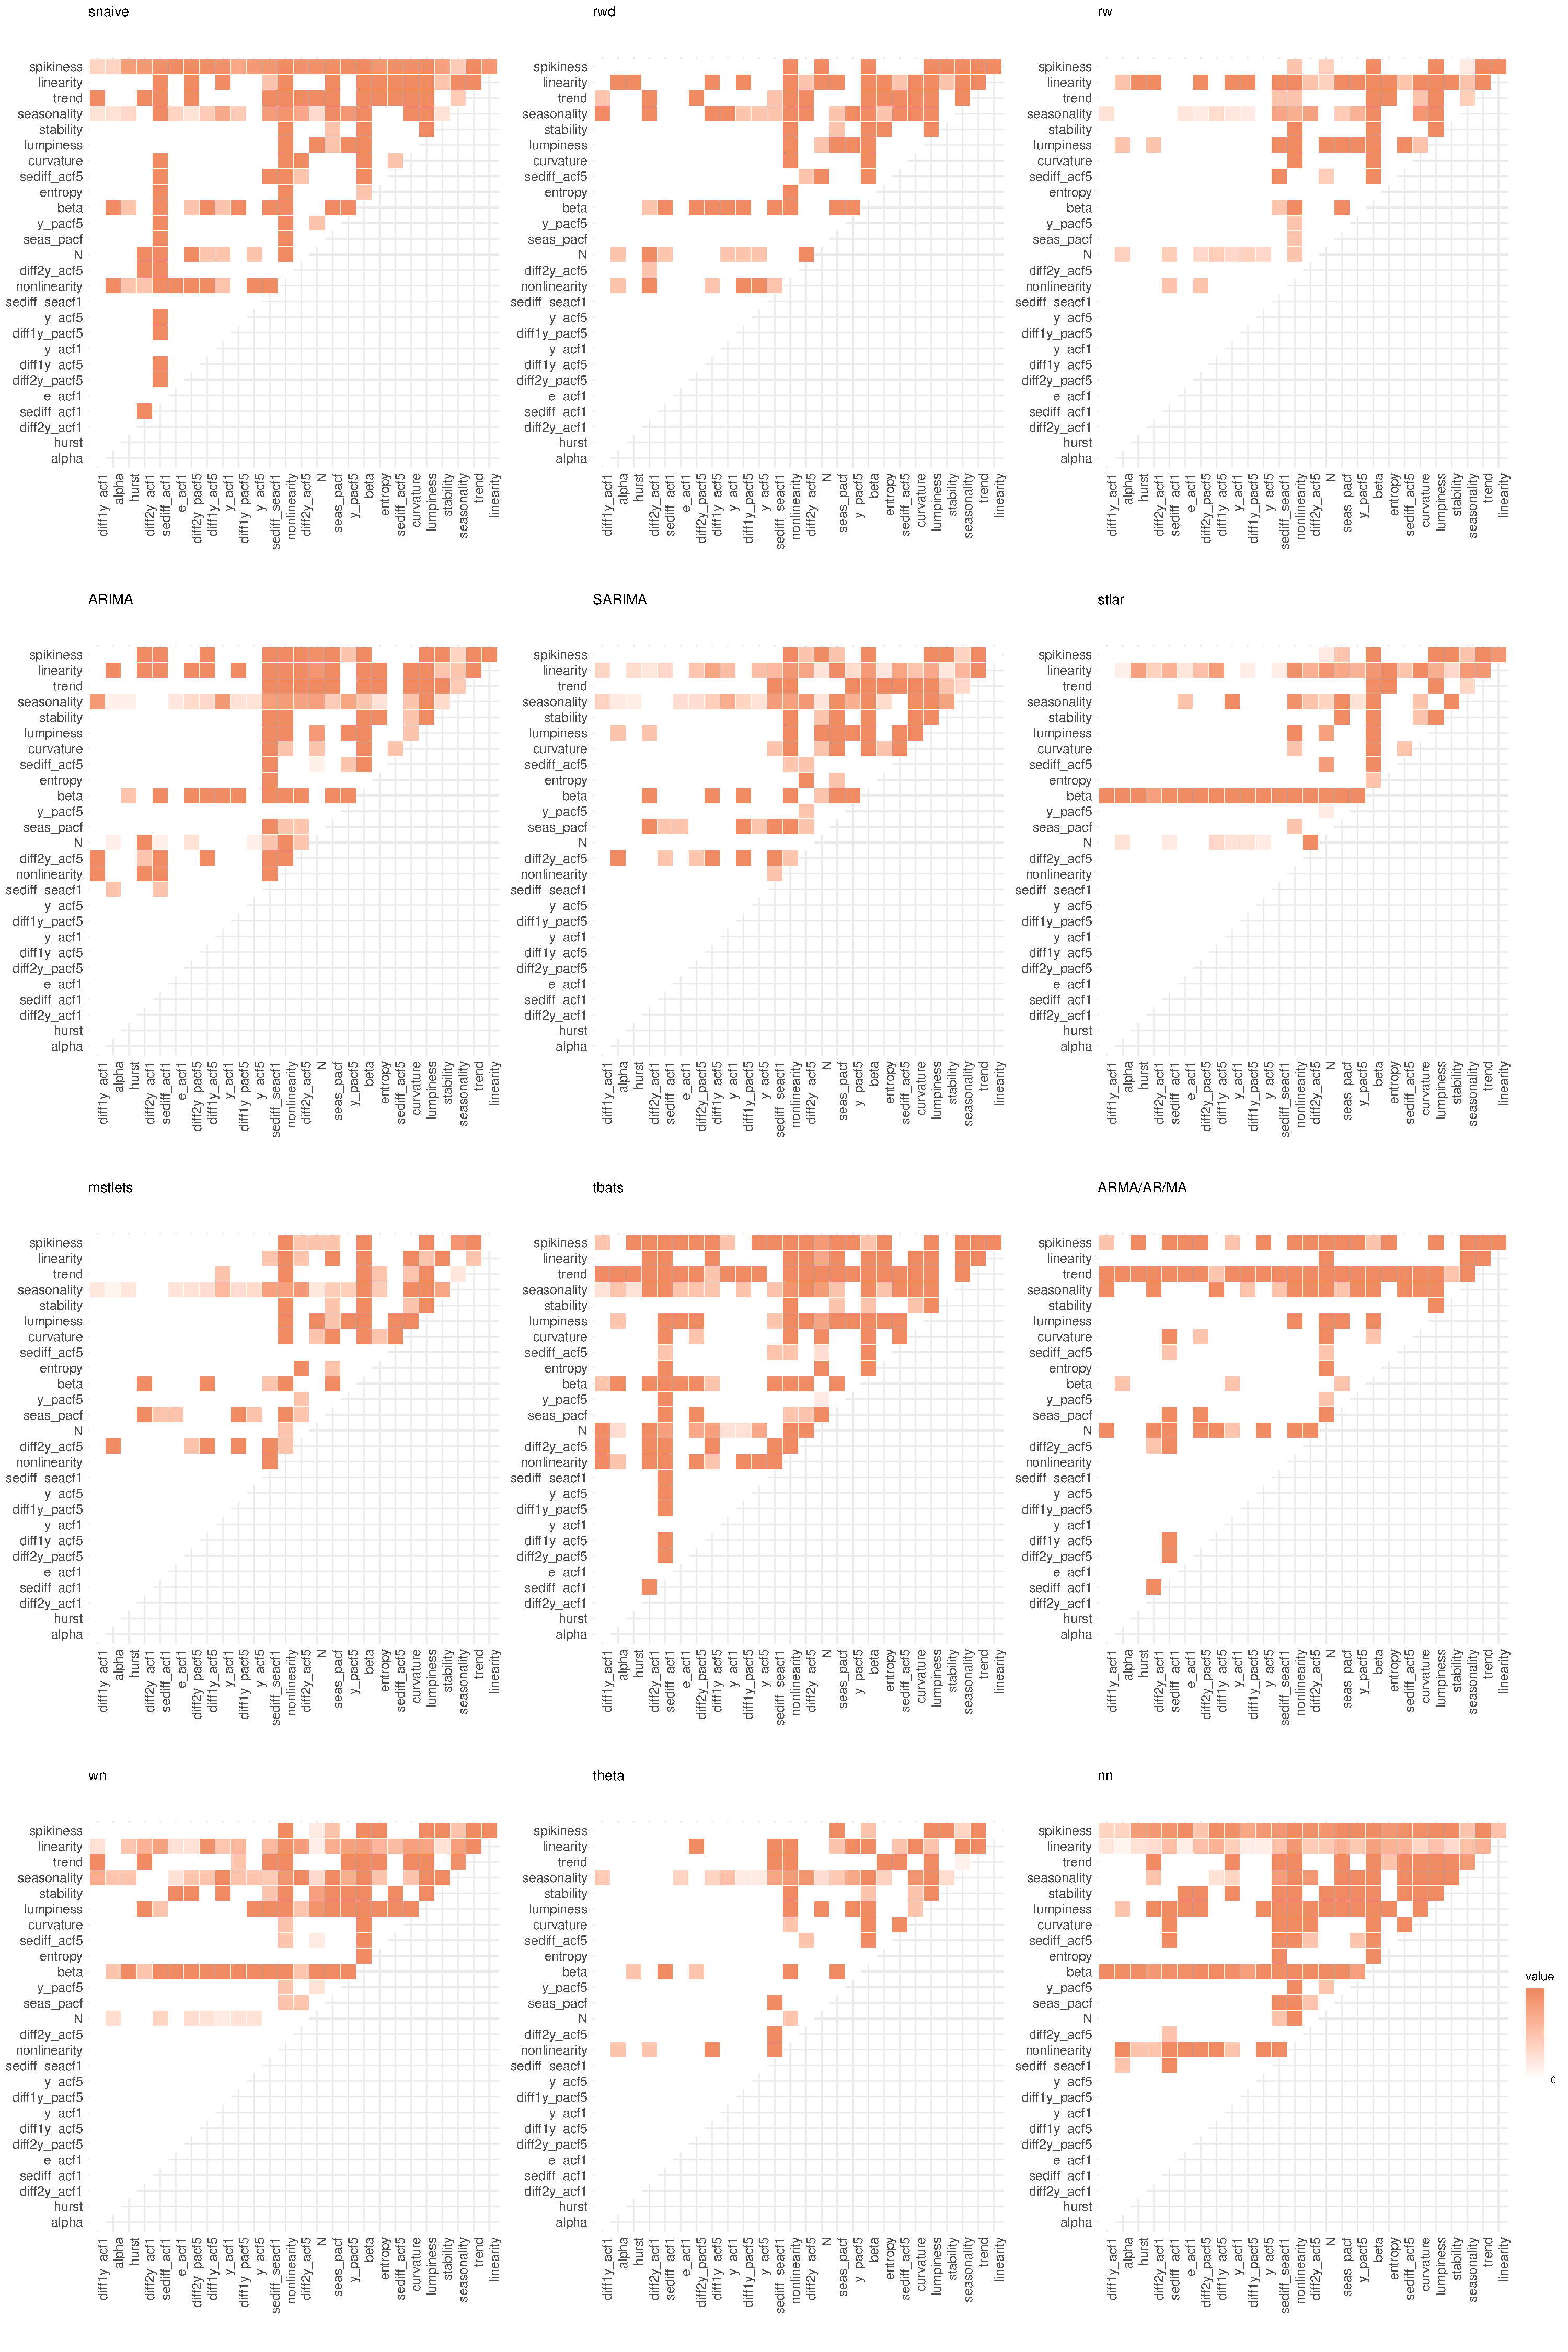
\includegraphics{figures/friedmanHW-1.pdf}
\caption{\label{fig:friedmanHW}Heat maps of relative strength of all
possible pairwise interactions calculated based on Friedman's
H-statistic for weekly series.}
\end{figure}

\subsection{Daily and Hourly data}\label{daily-and-hourly-data}

According to \autoref{fig:oobdailyhourly} the distributions corresponds
to observations that have been correctly classified dominate the top for
daily data. However, within daily series there are few observations that
have been incorrectly classified to tbats class with very high
probabilities. In general, neural network models have a higher chance of
getting selected for daily time series. Overall, for hourly series
random walk with drift models, tbats and neural network models have a
high chance of getting selected. Furthermore, it is important to note
that all hourly series have been assigned a non-zero probability of
getting selected to neural network class.

Variable importance graph for daily and hourly data are shown in
\autoref{fig:vidaily} and \autoref{fig:vihourly} respectively. The most
important features for daily time series are, strength of seasonality
corresponds to the weekly seasonality (7, measured by
seasonal\_strength1), stability, trend, lumpiness and linearity.
Furthermore, length of the series is important in determining random
walk, random walk with drift, mstlarima, mstlets, stlar, theta and nn
classes.

According to \autoref{fig:vihourly}, the strength of daily seasonality
(period=24, measured by seasonal\_strength1) appear to be more important
than the strength of weekly seasonality (period=168, measured by
seasonal\_strength2). Furthermore, entropy, linearity, sum of squares of
first 5 coefficients of PACF, curvature, trend, spikiness and stability
were found to be the most important features in determining best
forecasting method for hourly time series. Only snaive category ranked N
among top 5 for hourly time series. The strength of weekly seasonality
also seems to be one of the most important features for classes snaive,
random walk, mstlarima, and tbats.

\autoref{fig:dailypdp} shows the partial dependency plots of the top 3
features for daily series. According to the results of
\autoref{fig:dailypdp} shorter series tends to select random walk with
drift models while probability of selecting snaive, mstlarima and
mstlets models increases as the length of series increases. Neural
network models show a non-monotonic relationship with length of the
series (N). The theta models tend to be selected for series with high
annual seasonality but very low weekly seasonality.

The partial dependency plots of the top 3 features for hourly series are
shown in \autoref{fig:hourlypdp}. According to \autoref{fig:hourlypdp}
the probability of selecting random walk, random walk with drift, theta
model and white noise process decrease with higher value of strength of
daily (seasonal\_strength1) seasonality, while the opposite relationship
holds for the other classes. On the other hand, probability of selecting
random walk model increase as the strength of weekly seasonality
increases.

\begin{figure}
\centering
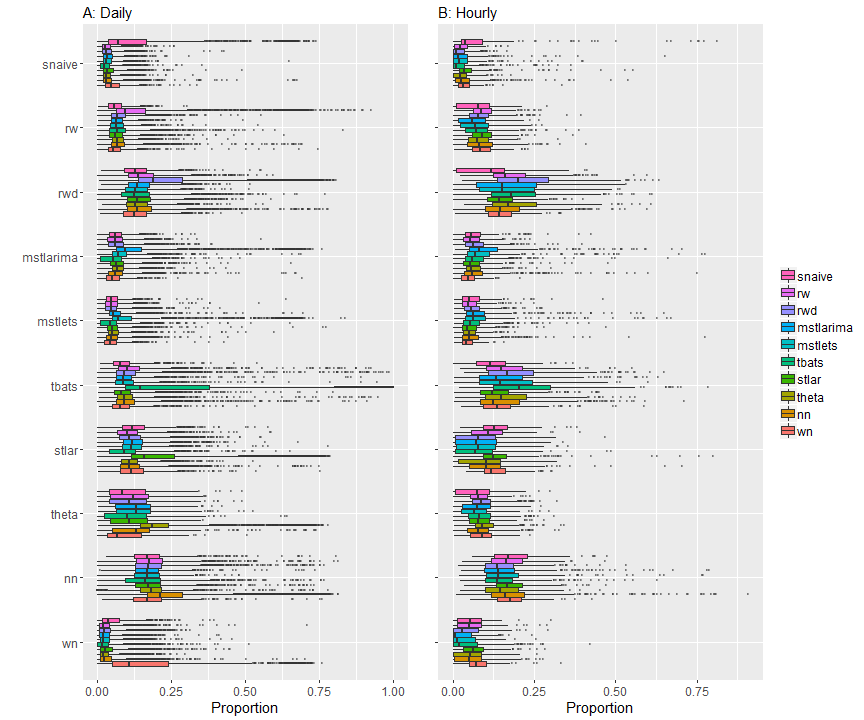
\includegraphics{figures/oobdailyhourly-1.png}
\caption{\label{fig:oobdailyhourly}Visualization of the vote matrix based on
OOB sample for daily and hourly random forests. The Y-axis denotes what
was predicted from the random forest. The X-axis denotes the proportion
of times each time series was classified to each class. The colours of
boxplots corresponds to class label of the ``best'' forecast-model
identified based on MASE and sMAPE. On each row, distribution of
correctly classified class dominates, indicating a good classification
of the meta-learners.}
\end{figure}

\newpage

\begin{figure}[h]

{\centering 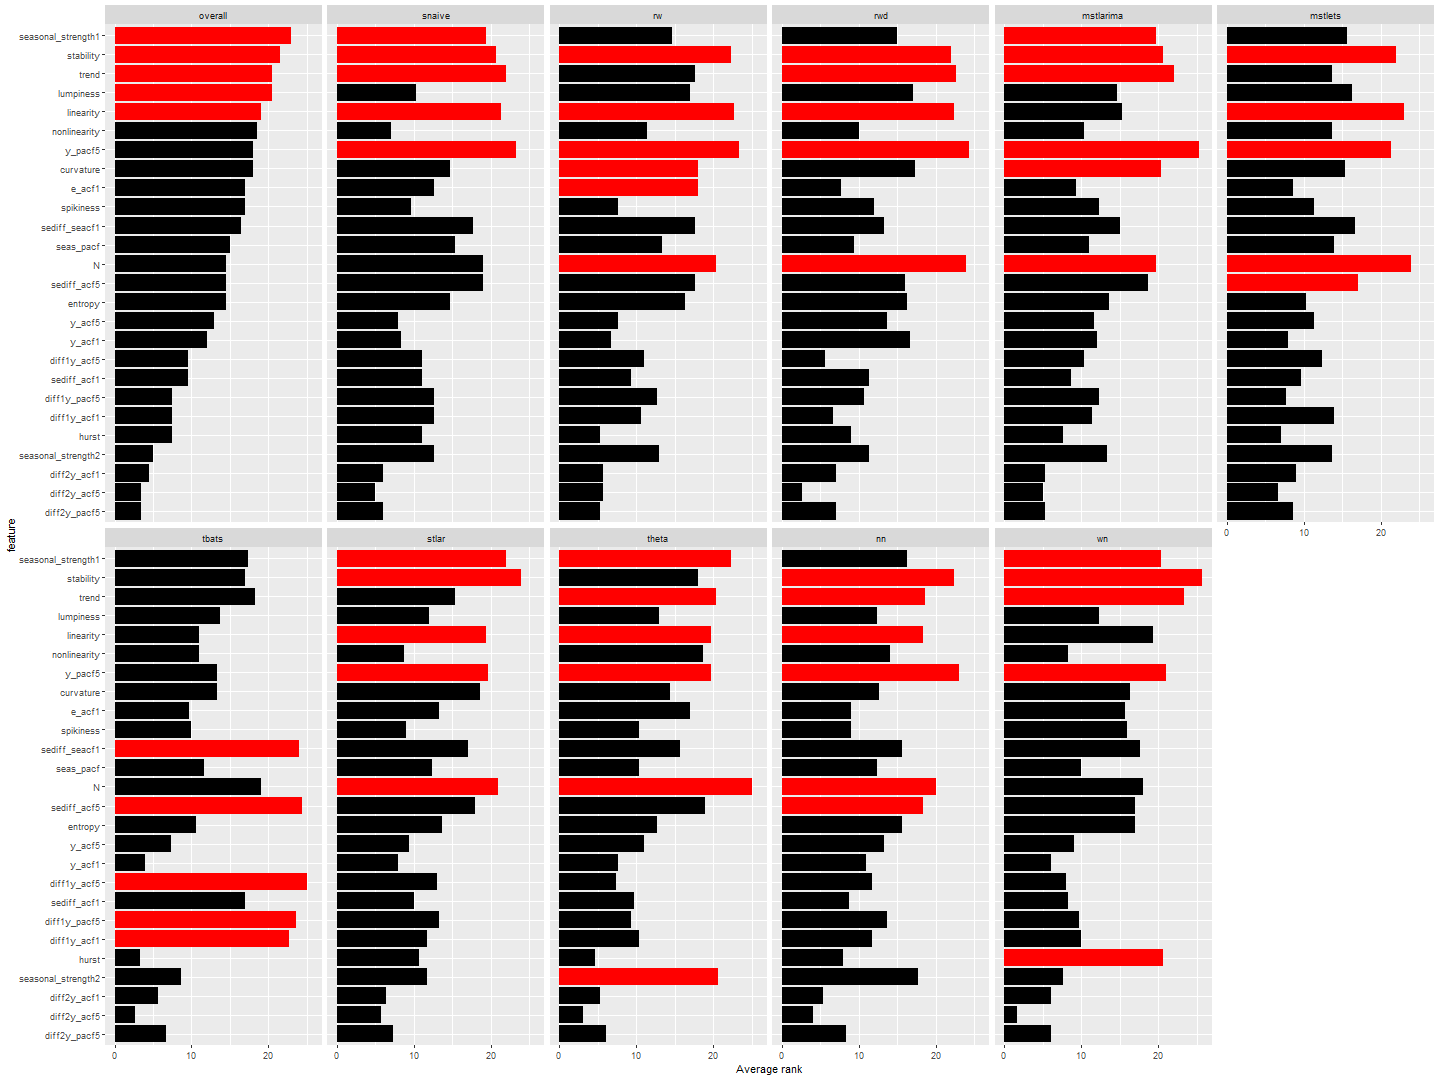
\includegraphics{figures/vidaily-1} 

}

\caption{Feature importance plot for daily data. Permutation-based VI measure and mean decrease in Gini coefficients are used to evaluate overall feature importance. Class-specific feature importance is evaluated based on the three measures: permutation-based VI, PD-based VI measure, and ICE-based VI measure. Longer bars indicate more important features. Top 5 features are highlighted in red.}\label{fig:vidaily}
\end{figure}

\begin{figure}
\centering
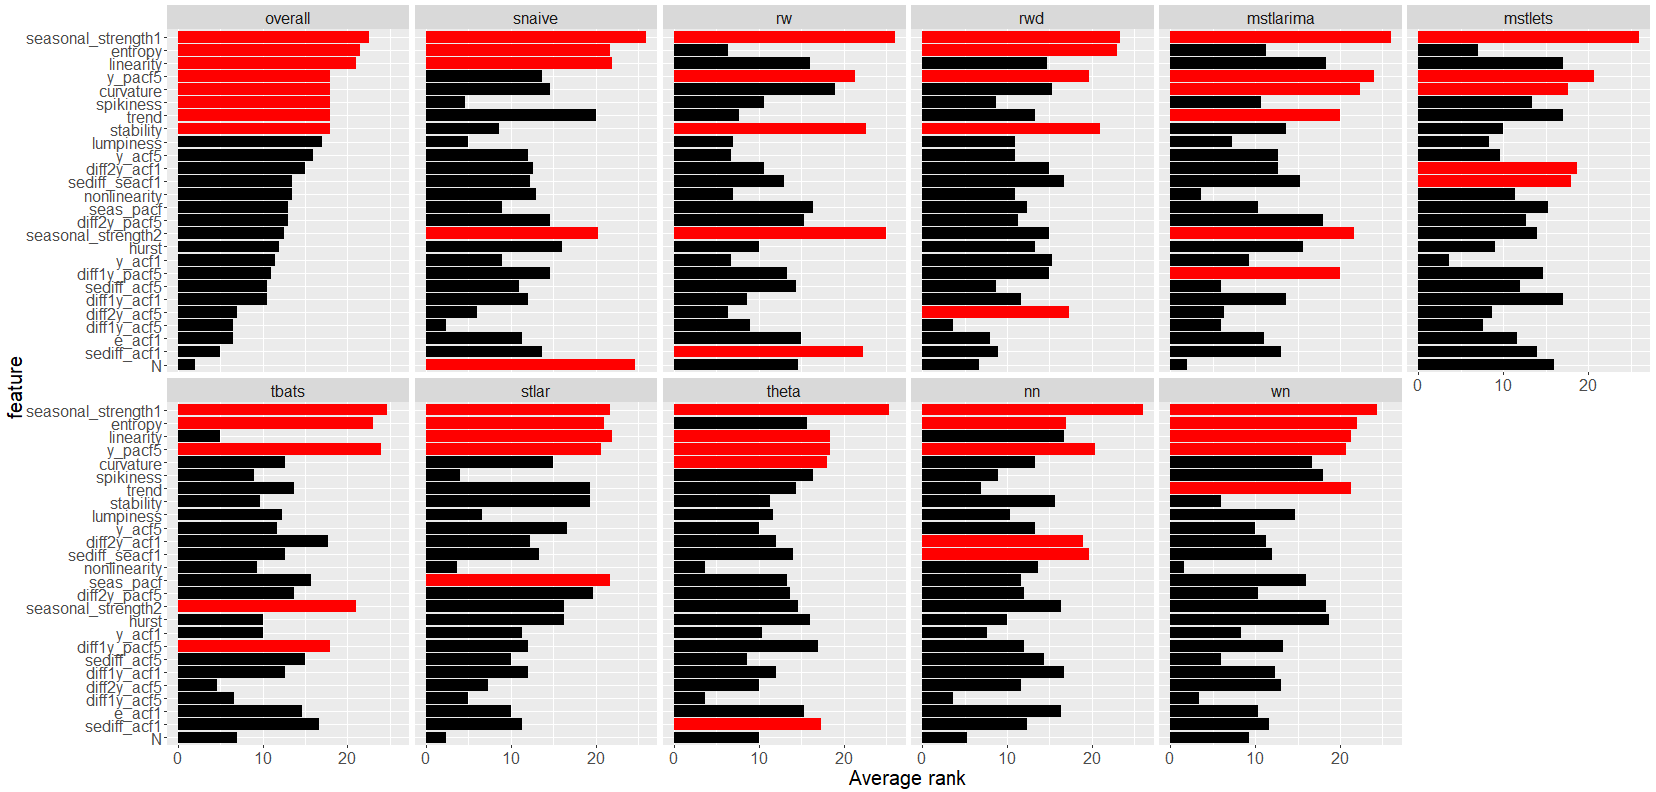
\includegraphics{figures/vihourly-1.png}
\caption{\label{fig:vihourly}Feature importance plot hourly series.
Permutation-based VI measure and mean decrease in Gini coefficients are
used to evaluate overall feature importance. Class-specific feature
importance is evaluated based on the three measures: permutation-based
VI, PD-based VI measure, and ICE-based VI measure. Longer bars indicate
more important features. Top 5 features are highlighted in red.}
\end{figure}

\newpage

\begin{figure}
\centering
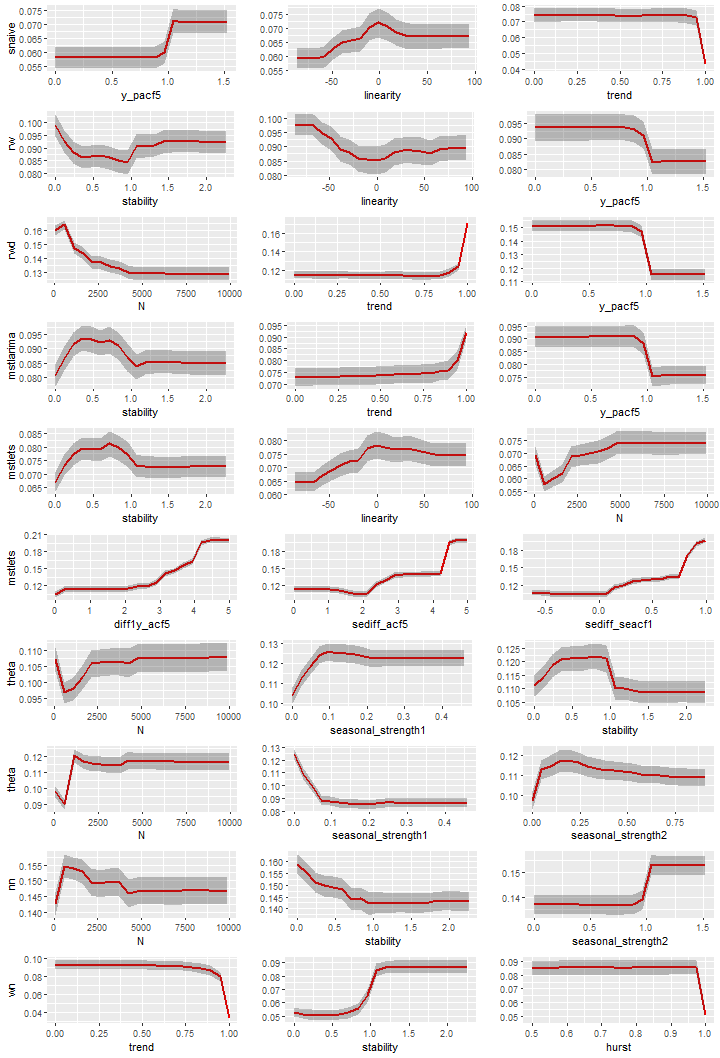
\includegraphics{figures/dailypdp-1.png}
\caption{\label{fig:dailypdp}Partial dependence plots for the top ranked
features based on variable importance measures (daily series). The
shading shows the 95\% confidence intervals. Y-axis denotes the
probability of belong to corresponding class. (seasonal\_strength1
denotes weekly seasonality and seasonal\_strength2 for annual
seasonality).}
\end{figure}

\newpage

\begin{figure}
\centering
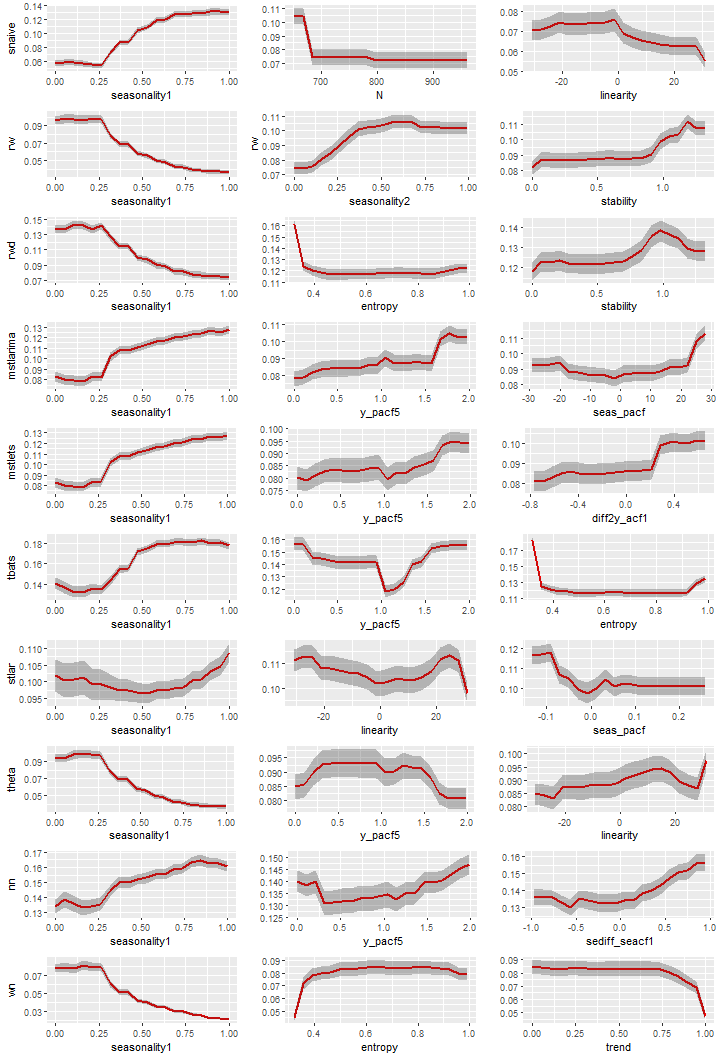
\includegraphics{figures/hourlypdp-1.png}
\caption{\label{fig:hourlypdp}Partial dependence plots for the top ranked
features from variable importance measures (hourly series). The shading
shows the 95\% confidence intervals. Y-axis denotes the probability of
belong to corresponding class. (seasonal\_strength1 denotes daily
seasonality and seasonal\_strength2 for weekly seasonality)}
\end{figure}

According to Friedman's H-statistic for daily series, sediff\_acf5 and
weekly seasonality (seasonal\_strength2) show high interactivity within
each class, while for hourly series sediff\_seacf1 and linearity show
high interactivity within each class. The partial dependency plots of
associated figures are shown in \autoref{fig:dtwopdp} and
\autoref{fig:htwopdp}. Each plot shows a unique pattern of interactivity
which is useful in separating one from another.

\begin{figure}
\centering
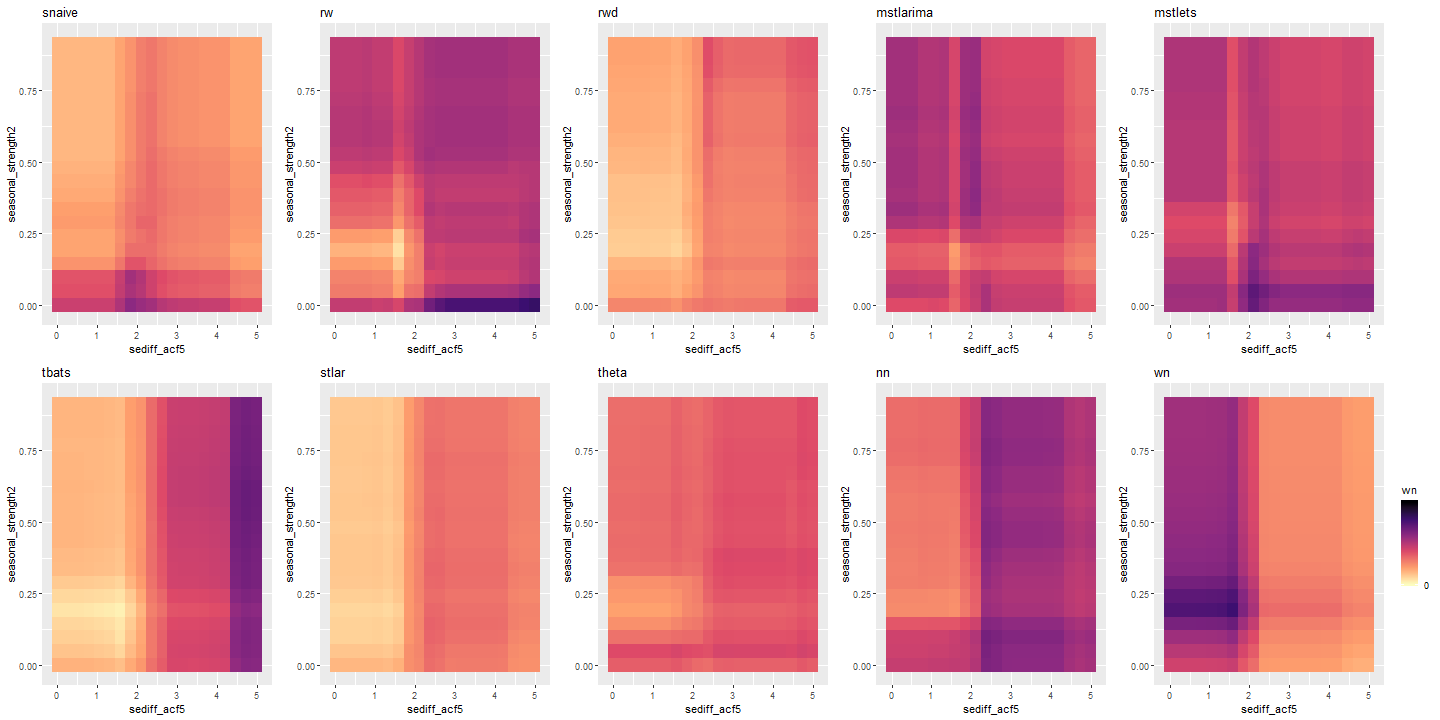
\includegraphics{figures/dtwopdp-1.png}
\caption{\label{fig:dtwopdp}Partial dependence plot of model selection
probability and the interaction of sediff\_acf5 and seasonal\_strength2
for daily data. Dark regions show the high probability of belonging to
the corresponding class shown in the plot title. Within each class
unique pattern of interaction pattern exist between sediff\_acf5 and
seasonal\_strength2.}
\end{figure}

\begin{figure}
\centering
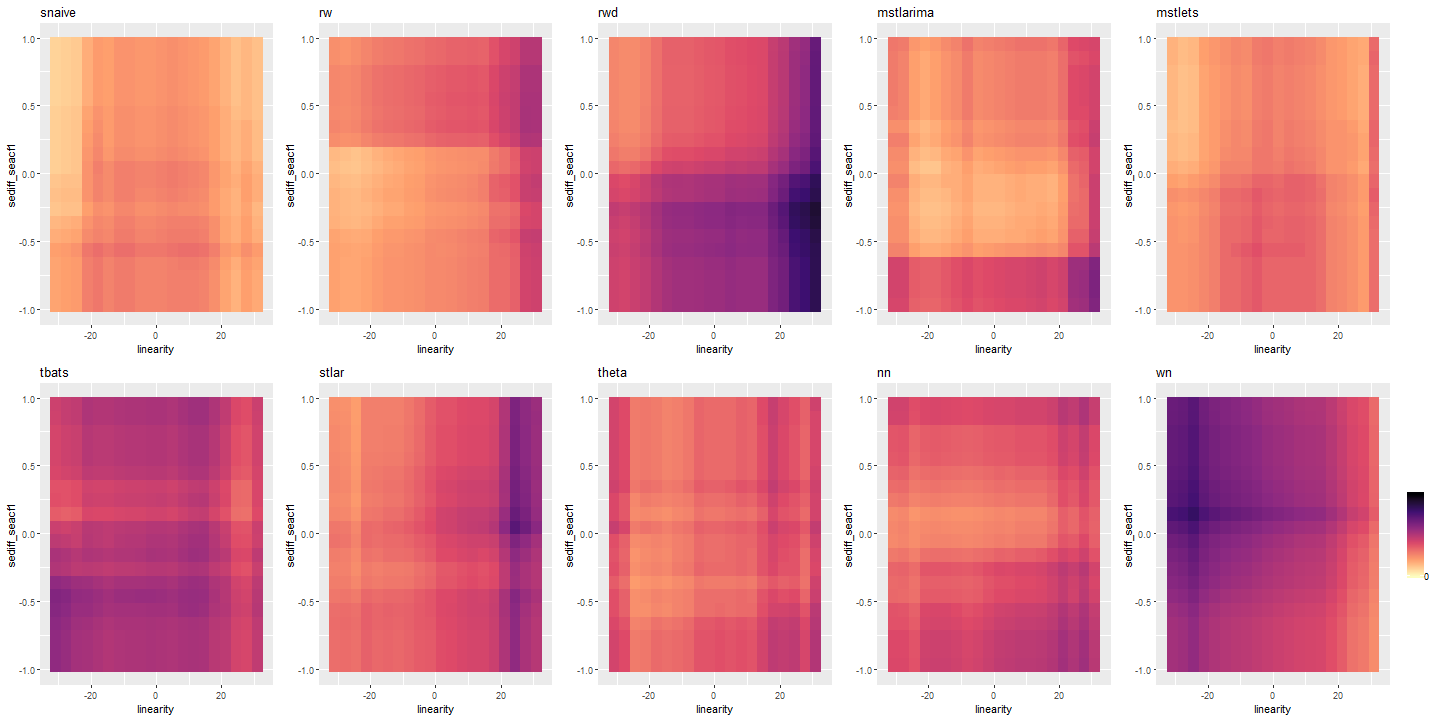
\includegraphics{figures/htwopdp-1.png}
\caption{\label{fig:htwopdp}Partial dependence plot of model selection
probability and the interaction of sediff\_seacf1 and linearity for
hourly data. Dark regions show the high probability of belonging to the
corresponding class shown in the plot title. Random walk and random walk
with drift class show opposite pattern of interactivity between
sediff\_seacf1 and linearity.}
\end{figure}

\clearpage

\subsection{Local Interpretable Model-agnostic
Explanations}\label{local-interpretable-model-agnostic-explanations}

\begin{figure}[h]

{\centering 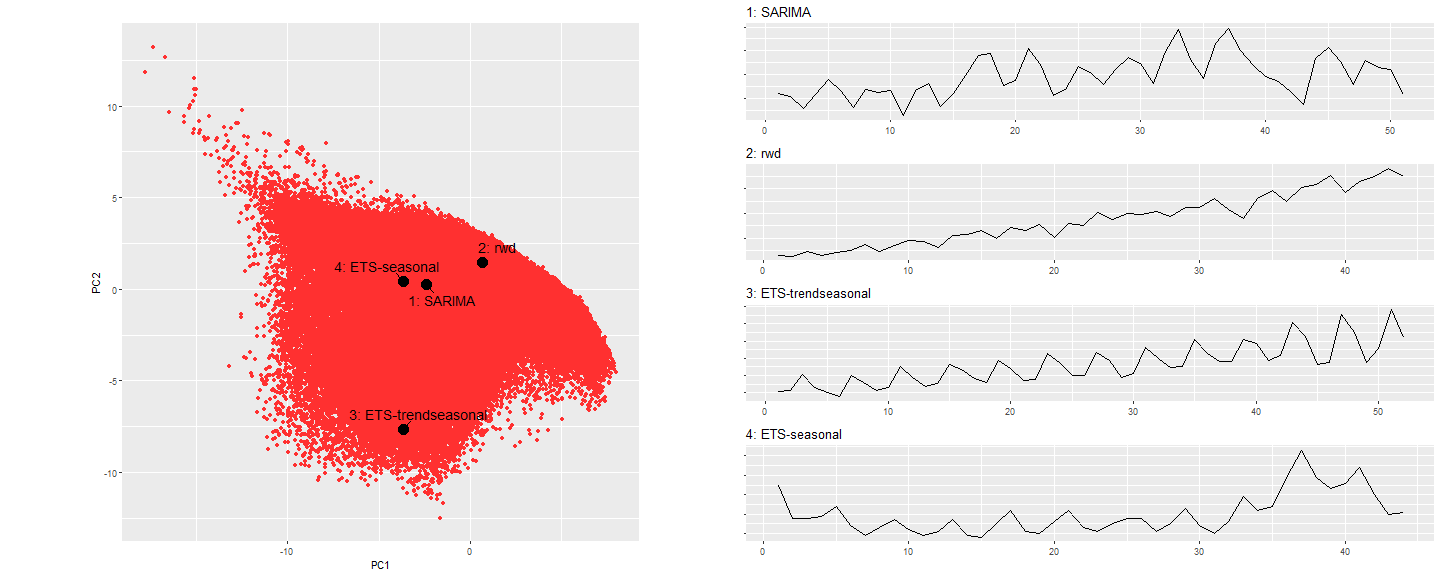
\includegraphics{figures/quarterlylime-1} 

}

\end{figure}

\begin{figure}[h]

{\centering 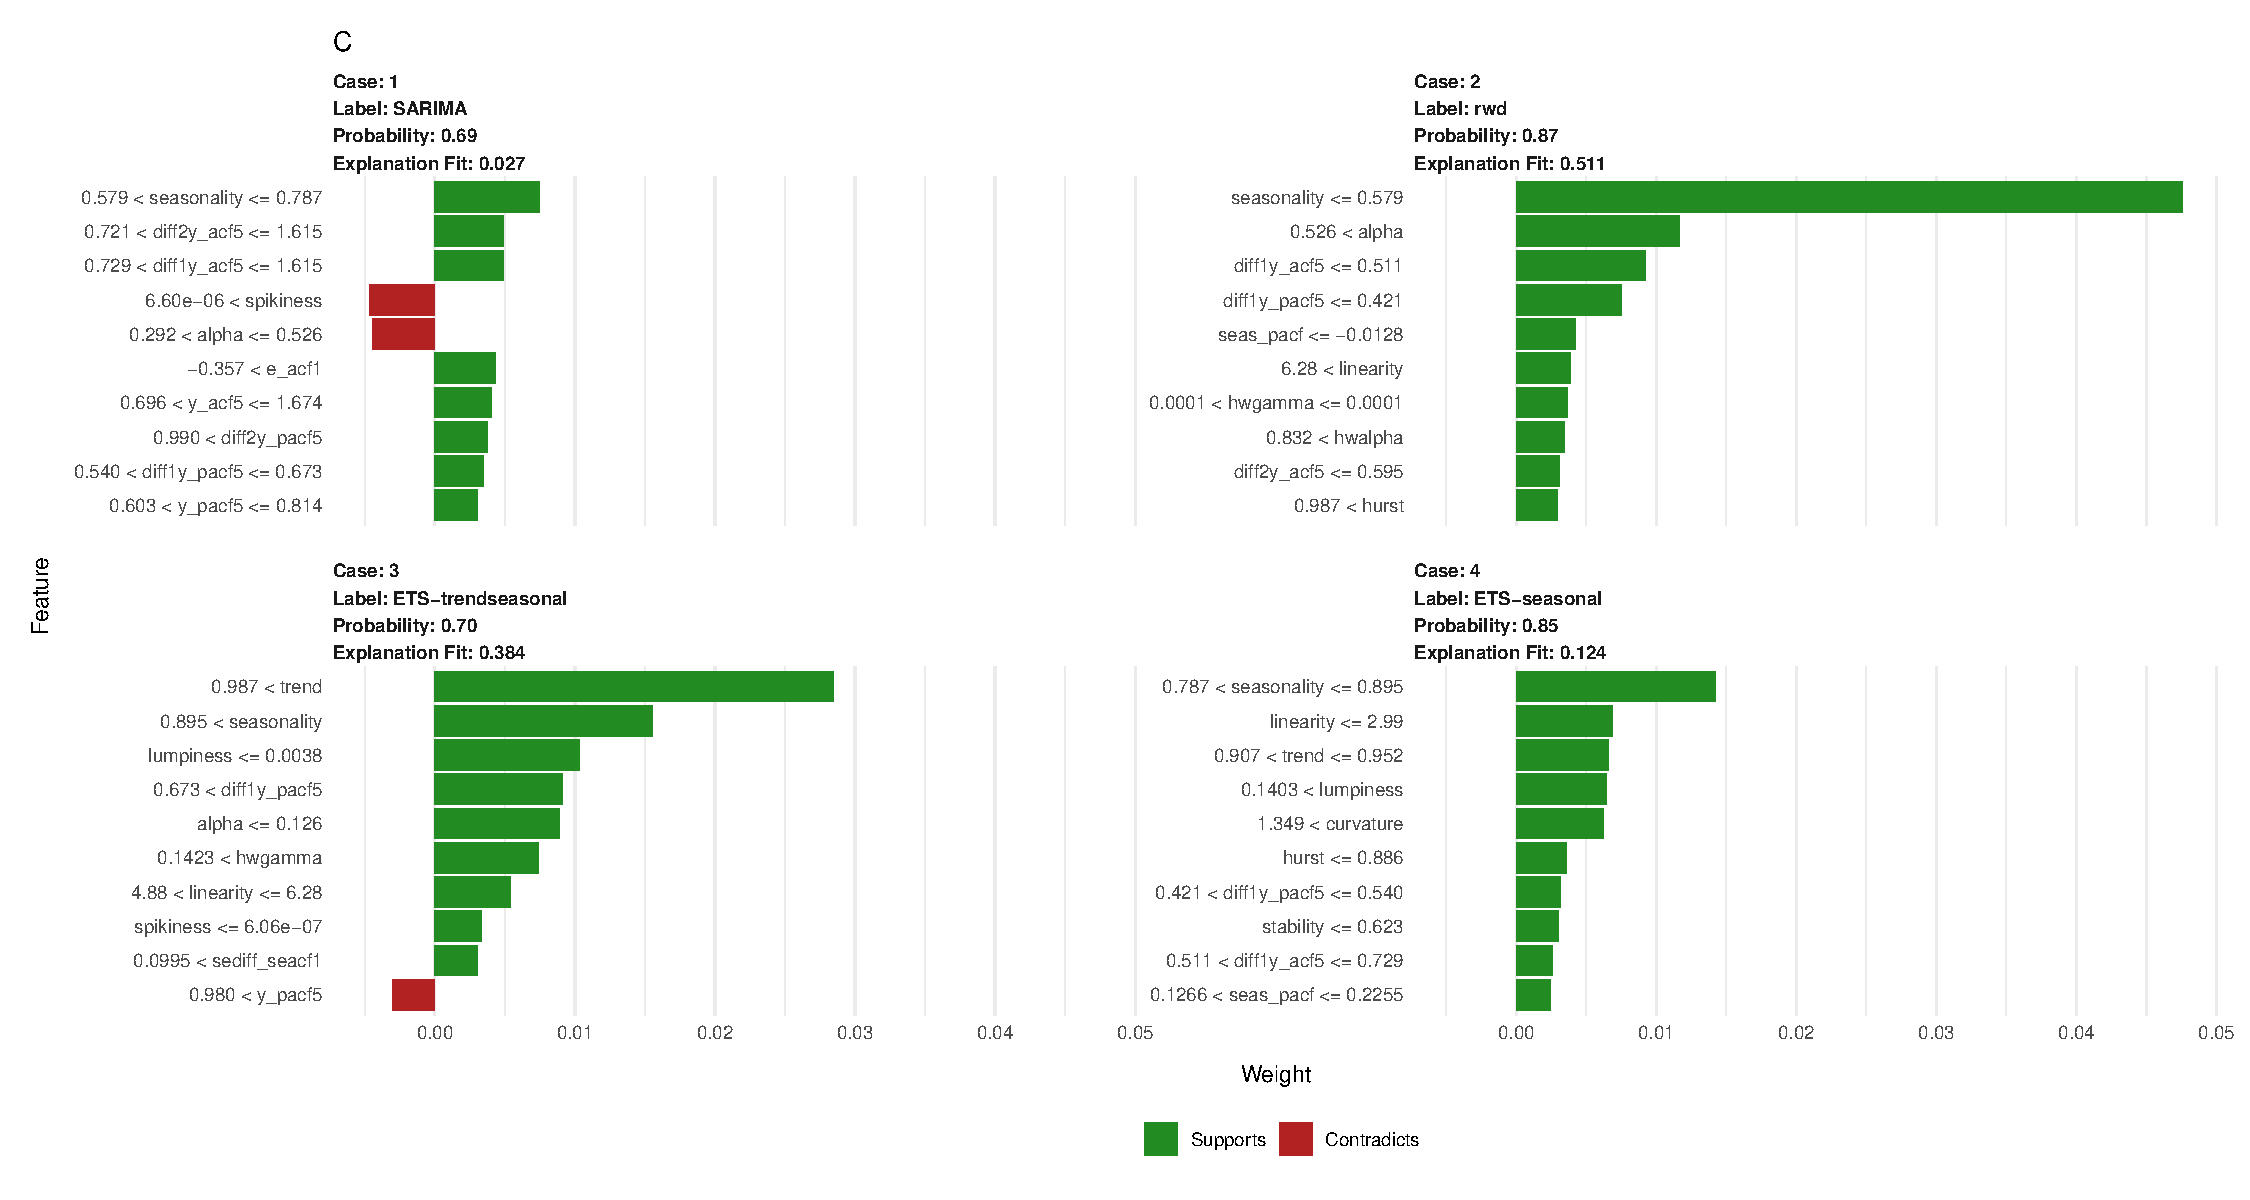
\includegraphics{figures/quarterlylime2-1} 

}

\caption{Panel A: Distribution of quarterly time series in the PCA space. Panel B: Time series corresponds to the highlighted points in the PCA space. Panel C: Local interpretable Model-agnostic explanations for four selected quarterly time series. Features denoted with green colour are supporting features for an outcome label and length of the bar is proportional to the weight of a feature.}\label{fig:quarterlylime2}
\end{figure}

We now illustrate how LIME approach can be used to zoom into local
regions of the data to identify which features, contribute most to
classify a specific instance. For the illustration we select four
different time series classified with high probability.
\autoref{fig:quarterlylime2} shows the feature contribution for the
instances highlighted on the PCA-space of quarterly series. We can see
how the strength of seasonality influences the FFORMS framework to
select different types of seasonal forecast-models. For example, SARIMA
model is selected when the seasonality varies between 0.579 and 0.787
(case 1), ETS-seasonal model is selected when the strength of
seasonality is greater than 0.787 (case 4), random walk with drift when
the seasonality is lower than 0.579 (case 2) and for the highly trended
and seasonal series (strength of seasonality \textgreater{} 0.895) ETS
model with a trend and seasonal component is selected (case 3). Further,
high value of diff1y\_acf5 in supports the selection of SARIMA for case
1 while, moderate value of diff1y\_acf5 supports the selection of
ETS-seasonal for the case 4. Similarly, we can explore the reasons for
other instances in all frequency categories. From LIME approach we can
gain insight into the local neighbourhood characteristics which lead to
the choice of a particular neighbourhood over alternative destinations.

\section{Discussion and Conclusions}\label{conclusions}

Forecast-model selection is both time and cost intensive process.
Consequently, the application of machine-learning approaches to predict
suitable forecast-model from a large number of potentially relevant time
series features is a topic growing popularity in the field of time
series forecasting. In this paper we use model-agnostic machine learning
interpretability tools to explore what is happening under the hood of
FFORMS framework and to gain an understanding of what features led to
the choices of FFORMS framework. The results we present here are a novel
application of machine learning interpretability methods to visualize
and explore the role of features in forecast-model selection.
Furthermore, explaining predictions is an important aspect in getting
humans trust and use the proposed framework effectively, if the
explanations are faithful and intelligible. Humans usually have prior
knowledge about the application domain, which they can use to accept
(trust) or reject prediction if they understand the reasons behind it.

\textcite{wickham2015visualizing} explain the importance of displaying
the ``model in the data space (m-in-ds)'' and ``data in the model space
(d-in-ms)''. Displaying the data in the model space (d-in-ms) is the
most commonly used approach for model-diagnostics. For example, plot of
fitted values versus residuals (\textcite{wickham2015visualizing}).
D-in-MS is a visualization of embedding high-dimensional data into a
low-dimensional space generated from the model. Visualization of D-in-MS
do not help to gain an understanding of the nature of the relationship
between features predicted outcome. In order to address this issue
\textcite{wickham2015visualizing} and \textcite{da2017interactive} have
highlighted the importance of visualizations of model in the data space.
In the context of classification, representation of m-in-ds could be
achieved by first, projecting the training data set into meaningful
low-dimensional feature space and then visualize the complete prediction
regions or their boundaries. In other words, this can be considered as
the visualization of predictor space in the context of the data space.
See \textcite{wickham2015visualizing} for visualization method of this
kind and \textcite{da2017interactive} for comparable method for random
forest algorithm.

We explore the role of features in two different perspectives: i)
individual effect, and ii) interaction effect. The features, strength of
trend, strength of seasonality, linearity, spikiness and curvature rank
among the top 10 within each frequency category.
\textcite{lemke2010meta} also pointed out features related to
nonstationarity and seasonality of a series are important factors for
choosing a forecast-models. Partial dependency plots are used to
visualize the learned relationship between features and the model
predictions. The displayed relationships confirm to domain knowledge
expectations. However, since several numbers of features are used to
build the framework with comparable contributions, and thus, all
individual contributions are small. Furthermore, our results show that
the performance of various methods depend upon the length of the time
series. Short time series tends to select simple methods such as random
walk models, snaive, etc. ETS models with both trend and seasonal
components, SARIMA models, mstl models tend to provide accurate
forecasts with longer time series as these are more parameterized
models.

As FFORMS framework is developed on top of random forest algorithm, it
takes into account every possible interaction. It was apparent from the
heat matrices of Friedman's H-Statistic that a substantial interaction
effect exists between the features. The strength of trend show a less
interactivity in yearly series data, reflecting that this feature is
more important on its own. The features involved in interaction and
their strength of interaction effect differ across the different
frequency categories (yearly, quarterly, monthly, weekly, daily and
hourly) as well as forecast-models (random walk, ETS models, etc.).
However, it is interesting to note that within each frequency category
all or a subset of ACF/PACF-based features interact with each other.
This confirms that the information regarding the correlation structure
of the time series is an essential information for the choice of model
selection.

Exploration of conditions learnt by the FFORMS framework also support
practitioners to make a good educated guess on suitable forecast-model
for a given problem. Further the results of this study is useful in
identifying new ways to improve forecasting accuracy by capturing
different features of time series.

\section{References}\label{references}

\section{Appendix}\label{appendix}

\subsection{Out-of-Bag Observations}\label{out-of-bag-observations}

\subsection{Votematrix calculation based on
OOB-observations}\label{votematrix-calculation-based-on-oob-observations}

\printbibliography

\end{document}
